\documentclass{article}
%Packages being imported that add functionality to LaTeX.
\usepackage[utf8]{inputenc}
\usepackage{geometry}
\usepackage{amssymb,amsmath,amsthm,mathtools,bussproofs,turnstile}
\usepackage{enumerate}
\usepackage{listings}
\usepackage{../common/vaucanson-g/vaucanson-g}
\usepackage{float}
\usepackage{epstopdf}
\usepackage{mathtools,array}
\usepackage{tcolorbox}
\usepackage[all]{xy}
\usepackage{xspace}
\SelectTips{cm}{10}     % Use the arrowheads that agree with inline arrows.
\everyxy={<2.5em,0em>:}
%Theorem Environments
\newtheorem{theorem}{Theorem}[section]
\newtheorem{lemma}[theorem]{Lemma}
\theoremstyle{definition}
\newtheorem{definition}{Definition}[section]
\newtheorem{corollary}[theorem]{Corollary}


%valuations
\newcommand{\valuations}{\ensuremath{\mathbb{V}}}
\newcommand{\propositions}{\ensuremath{\mathbb{P}}\xspace}
\newcommand{\proposition}{\ensuremath{p}\xspace}
%\newcommand{\acceptingState}{acc}
%\newcommand{\acceptingSymbol}{\alpha}
%\newcommand{\acceptingSymbols}{\beta}
\newcommand{\executionDef}{\ensuremath{\varepsilon=s_0, \actionLabel_0, s_1, \ldots}\xspace}
\newcommand{\execution}{\ensuremath{\varepsilon}\xspace}

%clts
\newcommand{\cltsDefIdx}[1]{\ensuremath{#1 = \lparen S_{#1},} \ensuremath{\Sigma_{#1}, \Delta_{#1},} \ensuremath{s_{0}^{#1}, \propositions_{#1}, \valuations_{#1}\rparen}\xspace}
\newcommand{\cltsDefShareSigmaIdx}[1]{\ensuremath{#1 = \lparen S_{#1},} \ensuremath{\Sigma, \Delta_{#1},} \ensuremath{s_{0}^{#1}, \propositions_{#1},} \ensuremath{\valuations_{#1}\rparen}\xspace}
\newcommand{\cltsDef}{\ensuremath{E = (S, \Sigma, \Delta, s_{0}, \propositions, \valuations)}\xspace}
\newcommand{\cltsEmbeddingDef}[1]{\ensuremath{clts(#1) = (S, \Sigma, \Delta, s_{0}, \valuations)}\xspace}
\newcommand{\automaton}[1]{\ensuremath{#1 = (S_{#1}, \Sigma_{#1}, \Delta_{#1}, s_{0}^{#1})}\xspace}
\newcommand{\labelSet}{\ensuremath{\mathcal{L}}\xspace}
\newcommand{\actionLabel}{\ensuremath{L}\xspace}
\newcommand{\action}{\ensuremath{l}\xspace}
\newcommand{\traces}{\ensuremath{\emph{Tr}}}

%composition
\newcommand{\cltsComposition}[3]{{\ensuremath{#1 \parallel_{#3} #2 = \lparen S,$ $\Sigma_{#1} \cup \Sigma_{#2},$ $\Delta,$ $(s_{0}^{#1},s_{0}^{#2}),$ $\propositions_{#1} \cup \propositions_{#2}$ $\valuations\rparen}}\xspace}
\newcommand{\ltsAdjustment}[2]{{\ensuremath{#1 \pm #2 = \lparen S_{#1}\times S_{#2},$ $\Sigma_{#1} \cup \Sigma_{#2},$ $\Delta,$ $(s_{0}^{#1},$ $s_{0}^{#2})\rparen}}\xspace}

%control problem
\newcommand{\controlSet}{\ensuremath{\mathcal{C}}}
\newcommand{\nonControlSet}{\ensuremath{\mathcal{U}}}
\newcommand{\controlProblemDef}{\ensuremath{\controlProblem =\langle E,$ $\controlSet,$ $\varphi \rangle}\xspace}
\newcommand{\controlProblem}{\ensuremath{\mathcal{I}}}

%GS
\newcommand{\gsV}{{\ensuremath{\mathcal{V}}}\xspace}
\newcommand{\gsX}{{\ensuremath{\mathcal{X}}}\xspace}
\newcommand{\gsY}{{\ensuremath{\mathcal{Y}}}\xspace}
\newcommand{\gsTheE}{\ensuremath{{\theta_e}}\xspace}
\newcommand{\gsTheS}{\ensuremath{{\theta_s}}\xspace}
\newcommand{\gsRhoE}{\ensuremath{{\rho_e}}\xspace}
\newcommand{\gsRhoS}{\ensuremath{{\rho_s}}\xspace}

%FDS
\newcommand{\enumSet}[1]{\#(#1)}
\newcommand{\enumSetDef}{$\#:\mathcal{P}(\mathcal{M})\mapsto [0\ldots2^{|\mathcal{M}|}-1]$\xspace}
\newcommand{\fdsDefIdx}[1]{$#1= \langle \gsV_{#1},$ $\theta_{#1},$ $\rho_{#1},$ $\mathcal{J}_{#1},$ $\mathcal{C}_{#1}\rangle$\xspace}
\newcommand{\fdsD}{\ensuremath{\mathcal{D}}\xspace}
\newcommand{\fdsDef}{$\fdsD = \langle \gsV_d,$ $\theta_d,$ $\rho_d,$ $\mathcal{J}_d,$ $\mathcal{C}_d\rangle$\xspace}
\newcommand{\fdsControlProblemDef}{\ensuremath{\fdsControlProblem =\langle \gsX,} \ensuremath{\gsY,$ $\varphi \rangle}\xspace}
\newcommand{\fdsControlProblem}{\ensuremath{\mathcal{K}}\xspace}
%realizability theorems
\newcommand{\varState}[1]{\ensuremath{\hat{s}_{#1}}\xspace}
\newcommand{\varLabel}[1]{\ensuremath{\hat{l}_{#1}}\xspace}
\newcommand{\varphiLTL}{\ensuremath{\varphi_{FDS}}\xspace}
\newcommand{\varphiLTLDef}{\ensuremath{\varphiLTL = (\theta_e \implies \theta_s) \wedge (\theta_e \implies \square((\boxdot \rho_e) \implies \rho_s)) \wedge (\theta_e \wedge \rho_e \implies val(\varphi))}\xspace}
\newcommand{\varphiCLTS}{\ensuremath{\varphi_{CLTS}}}
\newcommand{\varphiCLTSDef}{\ensuremath{\varphiCLTS = ()}\xspace}
\newcommand{\varphiLtlFormula}{\ensuremath{(\theta_e \implies \theta_s) \wedge (\theta_e \implies \square((\boxdot \rho_e) \implies \rho_s)) \wedge (\theta_e \wedge \rho_e \implies val(\varphi))}}
\newcommand{\fdsEmbeddingDef}{\ensuremath{ltl(\controlProblem) = \langle \gsX,$ $\gsY,$ $\varphiLTL \rangle}\xspace}
\newcommand{\fdsEmbedding}{\ensuremath{ltl(\controlProblem)}\xspace}
\newcommand{\cltsCPEmbeddingDef}{\ensuremath{clts(\fdsControlProblem) =\langle E,$ $\controlSet,$ $\varphiCLTS \rangle}\xspace}
\newcommand{\cltsCPEmbedding}{\ensuremath{clts(\fdsControlProblem)}\xspace}


%formulae
\newcommand{\true}{\emph{true} }
\newcommand{\false}{\emph{false} }
\newcommand{\assume}{\phi}
\newcommand{\guarantee}{\gamma}
\newcommand{\invariant}{\rho}
\newcommand{\fluentp}[1]{\dot{#1}}
\newcommand{\fluent}{\emph{fl}}
\newcommand{\set}[1]{\{#1\}}
\newcommand{\gr}{{GR(1)}\xspace}
\newcommand{\sgr}{{SGR(1)}\xspace}
\newcommand{\G}{{\bf G}}
\newcommand{\F}{{\bf F}}
\newcommand{\X}{{\bf X}}
\newcommand{\U}{{\bf U}}


\title{Concurrent Labeled Transition Systems (CLTS)} %Change this to the appropriate number.
\author{Fundamentals} %Change this to your name.
\date{}

\begin{document}


\maketitle

%Counters for setting the appropriate numbering.
\setcounter{section}{1} %This gives the chapter number.
\setcounter{theorem}{1} %This gives the item number.
%Note that the item number should be one less than you desire..

\subsection{Concurrent Labeled Transition Systems (CLTS)}
\begin{definition}
	\actionLabel{def:CLTS} \emph{(Concurrent Labelled Transition Systems)} 
	A \emph{Concurrent Labelled Transition System} (CLTS) is defined as \cltsDef, where $S$ is a finite set of states, $\Sigma$ is its {\em set of actions}, $\Delta \subseteq (S \times 2^{|\Sigma|} \times S)$ is a transition relation, $s_0 \in S$ is the initial state, $\propositions : \{\proposition_0,\ldots,\proposition_k\}$ is a finite set of atomic propositions and $\valuations : S \mapsto  2^{|\propositions|}$ is the function that defines the set of propositions ¨that hold at a given state $s \in S$.  
	%We denote $\Delta(s)=\{\actionLabel~|~(s,\actionLabel,s') \in \Delta\}$. 
	A CLTS is deterministic if $(s,\actionLabel,s')$ and $(s,\actionLabel,s'')$ are in $\Delta$ then $s'=s''$ should hold.
	An execution of $E$ is a word \executionDef where $(s_i, \actionLabel_i, s_{i+1}) \in \Delta$. 
	%A word $\pi$ is a trace (induced by $\varepsilon$) of $E$ if its the result of removing every $s_i$ from an execution $\varepsilon$ of $E$. 	We denote the set of infinite traces of $E$ by $\traces(E)$. 
	Given a transition $(s_i, \actionLabel, s_j) \in \Delta$, we will call $\actionLabel$ its label, and each element $\action \in \actionLabel$ an action.
\end{definition}

\subsection{LTL satisfaction over CLTS}

%~\cite{DBLP:conf/sigsoft/GiannakopoulouM03}. 

A LTL formula is defined inductively using the standard Boolean connectives and temporal operators $X$~(next), $U$ (strong until) as follows: 
$\varphi ::= \proposition \mid \neg \varphi \mid \varphi \vee \psi \mid \X \varphi \mid \varphi U \psi,$
where $\proposition$ is an atomic proposition from $\propositions$. 
As usual we introduce $\wedge$, $\F$ (eventually), and $\G$ (always) as syntactic sugar. 
Let $\epsilon$ be the set of infinite executions over $\Delta$.
The execution \executionDef satisfies $\proposition$ at position $i$ (we are only considering states, not labels, when defining the position), denoted $\execution,i \models \proposition$, if and only if the state $s_j$ at position $i$ in $\execution$ (i.e. $\execution_i = s_j$)  satisfies $\proposition \in \valuations(s_i)$.


Given an infinite execution $\execution$, the satisfaction of a formula $\varphi$ at position $i$, denoted $\execution,i\models\varphi$, is defined as follows:

\begin{tabular}{ l c l }
$\execution, i \models_d \proposition$ & $\triangleq$ & $\proposition \in \valuations(\execution_i)$\\
$\execution, i \models_d \neg \varphi$ & $\triangleq$ & $\execution, i \not\models_d \varphi$\\
$\execution, i \models_d \varphi \vee \psi$ & $\triangleq$ & $(\execution, i \models_d \varphi) \vee (\execution, i \models_d \psi)$\\
$\execution, i \models_d \X \varphi$ & $\triangleq$ & $\execution, i +1 \models_d \varphi$\\
$\execution, i \models_d \varphi \U \psi$ & $\triangleq$ & $\exists j \geq i . \execution,j \models_d \psi \wedge \forall i \leq k \le k. \execution, k \models_d \varphi$\\
\end{tabular}
  
We say that $\varphi$ holds in $\execution$, denoted $\execution\models\varphi$, if $\execution,0\models\varphi$. 
A formula $\varphi \in \mbox{LTL}$ holds in an CLTS $E$ (denoted $E \models \varphi$) if it holds on every infinite execution produced by $E$.


%\subsection{CLTS fluent satisfaction}
%
We use linear temporal logics of fluents (FLTL) over CLTS models. %~\cite{DBLP:conf/sigsoft/GiannakopoulouM03}. 
A \emph{fluent} \emph{fl} is defined by a pair of sets and a Boolean value: $\emph{\fluent} = \langle I_{\emph{\fluent}}, T_{\emph{\fluent}}, \emph{Init}_{\emph{\fluent}} \rangle$, where $I_{\emph{\fluent}}\subseteq \mathcal{P}(Act)$ is the set of initiating actions, $T_{\emph{\fluent}} \mathcal{P}(Act)$ is the set of terminating actions and $I_{\emph{\fluent}}\cap T_{\emph{\fluent}}=\emptyset$. 
A fluent may be initially \true or \false as indicated by \emph{Init}$_{\emph{\fluent}}$. 
Every actions $\ell\in Act$ induces a fluent, namely $\fluentp{\ell}=\langle \{\ell\}, \{Act\setminus \set{\ell}\}, \false\rangle$. 
Finally, the alphabet of a fluent is the union of its terminating and initiating actions.

Let $\mathcal{F}$ be the set of all possible fluents over $\mathcal{P}(Act)$. 
An FLTL formula is defined inductively using the standard Boolean connectives and temporal operators $X$~(next), $U$ (strong until) as follows: 
$\varphi ::= \fluent \mid \neg \varphi \mid \varphi \vee \psi \mid \X \varphi \mid \varphi U \psi,$
where $\fluent\in\mathcal{F}$. 
As usual we introduce $\wedge$, $\F$ (eventually), and $\G$ (always) as syntactic sugar. 
Let $\Pi$ be the set of infinite traces over \emph{Act}.
The trace $\pi=\ell_0,\ell_1,\ldots$ satisfies a fluent $\emph{Fl}$ at position $i$, denoted $\pi,i \models \emph{Fl}$, if and only if one of the following conditions holds:
\begin{list}{-}%{\leftmargin=3em}
	\item $\emph{Init}_{\emph{Fl}} \wedge (\forall j \in \mathbb{N} \cdot 0 \leq j \leq i \rightarrow \nexists t \in T_{\fluent}: t \subseteq \ell_j)$
	\item $\exists j \in \mathbb{N} \cdot (j \leq i \wedge \exists i \in I_{\fluent}: i \subseteq \ell_j) \wedge (\forall k \in \mathbb{N} \cdot j < k \leq i \ \rightarrow \nexists t \in T_{\fluent}: t \subseteq \ell_k)$
\end{list}

Given an infinite trace $\pi$, the satisfaction of a formula $\varphi$ at position $i$, denoted $\pi,i\models\varphi$, is defined as follows:

\begin{tabular}{ l c l }
$\pi, i \models_d \neg \varphi$ & $\triangleq$ & $\pi, i \not\models_d \varphi$\\
$\pi, i \models_d \varphi \vee \psi$ & $\triangleq$ & $(\pi, i \models_d \varphi) \vee (\pi, i \models_d \psi)$\\
$\pi, i \models_d \X \varphi$ & $\triangleq$ & $\pi, i +1 \models_d \varphi$\\
$\pi, i \models_d \varphi \U \psi$ & $\triangleq$ & $\exists j \geq i . \pi,j \models_d \psi \wedge \forall i \leq k \le k. \pi, k \models_d \varphi$\\
\end{tabular}
  
We say that $\varphi$ holds in $\pi$, denoted $\pi\models\varphi$, if $\pi,0\models\varphi$. 
A formula $\varphi \in \mbox{FLTL}$ holds in an CLTS $E$ (denoted $E \models \varphi$) if it holds on every infinite trace produced by $E$.
A \emph{fluent} \fluent \space is defined by a set of initiating actions $I_{\fluent}$, a set of terminating actions $T_{\fluent}$, and an initial value \emph{Initially}$_{\fluent}$.

That is,
%\begin{equation*}
$ \fluent = \langle I_{\fluent}, T_{\fluent} \rangle_{\emph{initially}_{\fluent}} $, 
where 
$I_{\fluent},T_{\fluent} \subseteq \mathcal{P}(\emph{Act})$ 
and $I_{\fluent} \cap T_{\fluent} = \emptyset.$\\
%\end{equation*}
%A fluent may be initially \true or \false as indicated by the \emph{Initially}$_{\fluent}$ attribute,
%When we omit \emph{Initially}$_{\fluent}$, we assume the fluent is
%initially \emph{false}. We use $\fluentp{\ell}$ as short for the
%fluent defined as $\fluent = \langle \ell,
%\emph{Act}\setminus\set{\ell} \rangle$.
%Given the set of fluents $\Phi$, an FLTL formula is defined
%inductively using the standard boolean connectives and temporal
%operators $\mathbf{X}$ (next), $\mathbf{U}$ (strong until) as
%follows:\\
%%\begin{equation*}
%$\varphi ::= \fluent \mid \neg \varphi \mid \varphi \vee \psi \mid
%\mathbf{X} \varphi \mid \varphi \mathbf{U} \psi$,
%%\end{equation*}
%where $\fluent \in \Phi$.


%\subsection{FLTL $\rightarrow$ AccLTL}
%The first thing that will be addressed for a control problem $\mathcal{I} = \langle E, \mathcal{C}, \mathcal{F}, \varphi \rangle$ is the relation between fluent valuations and states in any given CLTS model. Assume $E = \langle S_E, \Sigma_E, \Delta_E, s^E_0 \rangle$ is the automaton that represents the plant, and $\mathcal{F}=\{fl_1,\ldots,fl_k\}$ with $fl_i = \langle I_i, T_i, init_i \rangle$ the set of fluents associated with a control problem. We will construct a new plant that is compatible with the valuation of the fluents at each step of the execution. To do this we construct an equivalent automaton for each fluent, compose them with each other and with the original plant $E$. If the plant was already compatible with the set of fluents, then its structure will remain unchanged. By constructing this fluent compatible plant in this way we have a simple mechanism to define the set of states satisfying any given fluent.  For each fluent $fl_i$ the related automaton is constructed as follows:
\[ FL_i = \langle S_{fl_i}, \Sigma_{fl_i}, \Delta_{fl_i}, s_{0_i}\rangle \]
Where:
\[S_{fl_i}= \{s^{\bot}_i, s^{\top}_i\} \]
\[\Delta_{fl_i} \text{is the minimal relation s.t.}\]
\[ \forall \alpha \in I_i: \{(s^{\bot}_i,\alpha,s^{\top}_i), (s^{\top}_i,\alpha,s^{\top}_i)\} \in \Delta_{fl_i} \]
\[ \forall \beta \in T_i: \{(s^{\top}_i,\beta,s^{\bot}_i), (s^{\bot}_i,\beta,s^{\bot}_i)\} \in \Delta_{fl_i} \]
\[
s_{0_i} = \begin{cases}
s^{\top}_i & init_i = \top \\
s^{\bot}_i & otherwise
\end{cases}
\]

The fluent compatible plant $E_G$ is the result of the synchronous parallel composition of the fluent automata with the original plant:
\[E_G = (E \parallel_s FL_1 ||_s \ldots ||_s FL_k) \]
And the function that determines which states satisfy which fluent is defined as:
\[ fl(i) = \{s \in S_{E_G} : s_{(i + 1)} = s^{\top}_i \} \]
Here $s_{(i+1)}$ stands for the state of the component $i+1$ of the parallel composition, with the original plant being the first one.
Atomic satisfaction of LTL formula $fl_i$ at step $j$ of trace $\pi$ can be redefined as:
\[ \pi_j \models fl_i \triangleq \pi_j \in fl(i) \]

We can prove that, for the trace $\pi=\ell_0,\ell_1,\ldots$, previous definition of satisfaction of fluent $fl_j$ at position $i$ is equivalent to $\ell_i \in fl(j)$.
From the definition:
\begin{itemize}%{\leftmargin=3em}
	\item $\emph{Init}_{\emph{Fl}} \wedge (\forall j \in \mathbb{N} \cdot 0 \leq j \leq i \rightarrow \nexists t \in T_{\fluent}: t \subseteq \ell_j)$
	\item $\exists j \in \mathbb{N} \cdot (j \leq i \wedge \exists i \in I_{\fluent}: i \subseteq \ell_j) \wedge (\forall k \in \mathbb{N} \cdot j < k \leq i \ \rightarrow \nexists t \in T_{\fluent}: t \subseteq \ell_k)$
\end{itemize} 

\subsection{CLTS composition}

When having to compose concurrent systems we define three different semantics that can be applied pairwise. Synchronous semantic $A ||_s B$ (Figure~\ref{fig:synchronous_composition})captures the composition of two components that share a single synchronizing event (implicit), where all participants should be able to make progress concurrently. The main motivation being digital components sharing a single clock. 
Asynchronous semantic $A ||_a B$ (Figure~\ref{fig:asynchronous_composition}) captures the interleaving interpretation of concurrency as found in LTS systems. 

\begin{figure}[h]
		\centering
	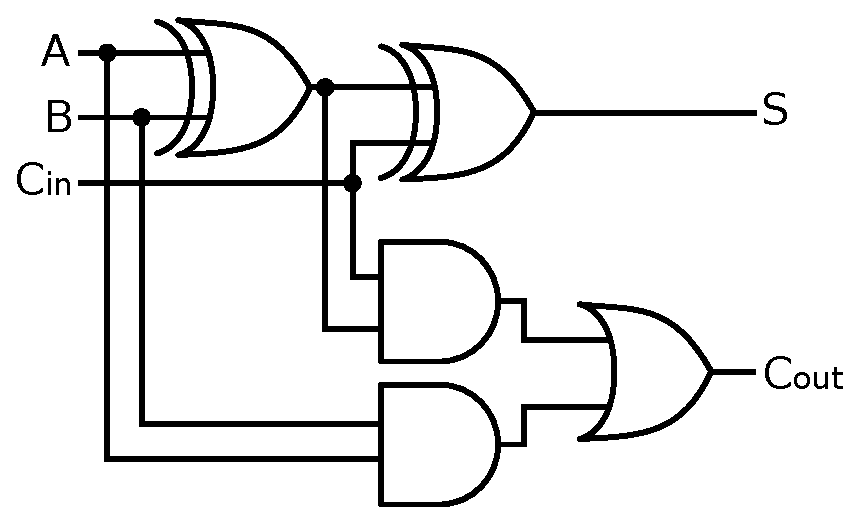
\includegraphics[scale=.4]{img/full-adder.eps}
	\caption{Full adder circuit}
	\label{fig:full_adder_circuit}
\end{figure}

A motivation for the synchronous composition can be found in the following example: a digital design consists of two 1 bit full adders working as separate units. Let $i \in \{1,2\}$ be the index of each adder and $a$ and $b$ the 1 bit entries to be added, $c\_in_i$ the incoming carry signal from another module, $s_i$ the output that represents the lower bit of the sum and $c_i$ the upper bit or carry out, then each 1 bit full adder can be modeled as a single state CLTS.  The FSP syntax would be the following:

\renewcommand{\ttdefault}{pcr}
\begin{figure}[H]
	\begin{lstlisting}[escapeinside={[*}{*]},basicstyle=\scriptsize\ttfamily,columns=flexible,mathescape=true,xleftmargin=3.0ex,keywordstyle=\textbf,morekeywords={if,while,do,else,fork,int,null, algorithm, is, input, output, return, for}]
	FULL_ADDER[i] = (<a[i],s[i]> -> FULL_ADDER[i] | <b[i],s[i]> -> FULL_ADDER[i] 
	| <c_in[i],s[i]> -> FULL_ADDER [i] | <a[i],b[i],c[i]> -> FULL_ADDER[i]
	| <a[i],c_in[i],c[i]> -> FULL_ADDER[i] | <b[i],c_in[i],c[i]> -> FULL_ADDER[i]
	| <a[i],b[i],c_in[i],s[i],c[i]> -> FULL_ADDER[i]| <> -> FULL_ADDER[i]).
\end{lstlisting}
%\caption{Game Structure to CLTS translation algorithm}
\label{fig:full_adder_fsp}
%%\vspace*{-4mm}
\MediumPicture
\end{figure}	

Applying asynchronous composition over single element labeled CLTS models ($FULL\_ADDER[1]$ $\parallel_{a}$ $FULL\_ADDER[2]$), would not properly capture the concurrent occurrence of signals, since it will not allow $<a_1,s_1,a_2,s_2>$ to happen.  

On the other hand, suppose that we are modeling the interaction of three processes $P_1$, $P_2$ and $receiver$ through a common buffer, $P_1$ produces either $a$ or $c$ and
$P_2$ produces either $d$ or $e$. $receiver$ will output a $x$ for each $a$ and a $y$ for each $d$. The FSP syntax would be the following:

\renewcommand{\ttdefault}{pcr}
\begin{figure}[H]
	\begin{lstlisting}[escapeinside={[*}{*]},basicstyle=\scriptsize\ttfamily,columns=flexible,mathescape=true,xleftmargin=3.0ex,keywordstyle=\textbf,morekeywords={if,while,do,else,fork,int,null, algorithm, is, input, output, return, for}]
	P_1 = (a->P_1 | c->P_1).
	P_2 = (d->P_2 | e->P_2).
	Receiver = (<a,x> -> Receiver | <d,y> -> Receiver | c -> Receiver | e -> Receiver).
	\end{lstlisting}
	%\caption{Game Structure to CLTS translation algorithm}
	\label{fig:receiver_fsp}
	%%\vspace*{-4mm}
	\MediumPicture
\end{figure}

Special attention is required when applying the parallel composition operator in order to recreate the system overall interaction. If synchronous semantic ($P_1\parallel_s P_2 \parallel_s receiver$) is to be applied then $receiver$ will not be able to synchronize with both $P_1$ and $P_2$ since at least one action on each component needs to be exercised. In this case, asynchronous composition ($P_1\parallel_a P_2 \parallel_a receiver$)will properly recreate the serialization of events coming from $P_1$ and $P_2$ through the buffer.

Composition semantics should be applied according the each domain, be aware that composition is not commutative if different semantics are applied for the same specification.

%Concurrent semantic $A ||_c B$ (Figure~\ref{fig:concurrent_composition}) captures the behavioral superset of the latter two. It can be used when composing two processes that may not share an implicit synchronizing event, as in the synchronous semantic, but can be observed by a third component that over samples the other two, allowing for the possibility of both concurrent an independent occurrence when observed as a composed system. A synthetic example is shown in Figure~\ref{fig:concurrent_systems}, motivation for this semantic can be found in clock domain crossing examples and micro architecture buffers.
%
%\begin{figure}[bt]
	\centering
	%\SmallPicture
	%\ShowFrame
		\begin{VCPicture}{(-3,-3)(3,2.5)}
			\SetStateLabelScale{1}
			\SetEdgeLabelScale{1}
			\State[1_a]{(-3,1.5)}{A}
			\State[1_b]{(-3,-1.5)}{B}			
			\State[1_c]{(2.5,0)}{C}						
			\Initial[n]{A}
			\Initial[n]{B}
			\Initial[w]{C}						
			%\ChgEdgeLineStyle{dashed} %\EdgeLineDouble
			%\ChgEdgeLineWidth{1.5}
			%\EdgeL{1}{2}{req}
			%\ArcR[.3]{6}{1}{reset}        
			\CLoopSW[.5]{A}{data_a}        
			%\CLoopSE[.5]{A}{idle_a}
			\CLoopSW[.5]{B}{data_b}        
			%\CLoopSE[.5]{B}{idle_b}				
			%\CLoopSW[.5]{C}{idle_c}        
			\CLoopSE[.5]{C}{data_b}					
			\CLoopNW[.5]{C}{data_a}					
			\CLoopNE[.5]{C}{<data_a,data_b,goal>}					
			%\RstEdgeLineWidth{1}
			%\RstEdgeLineStyle %\EdgeLineSimple
			%\EdgeL{2}{3}{grant}
			%\EdgeL[.75]{2}{5}{\overline{grant}}
			%\VArcR{arcangle=-20}{3}{6}{timeout}
			%\ArcR[.6]{3}{6}{timeout}
			%\ArcL{5}{1}{hready}
			%\VArcR{arcangle=-30}{3}{4}{hready}
		\end{VCPicture}

	\caption{A, B and C systems}
	\label{fig:concurrent_systems}
	%%\vspace*{-4mm}
	\MediumPicture
\end{figure}
\begin{figure}[bt]
	\centering
\minipage{0.32\textwidth}	
\centering
	%\SmallPicture
	%\ShowFrame
	\begin{VCPicture}{(-1.5,-1.5)(1.5,1.5)}
		\SetStateLabelScale{.8}
		\SetEdgeLabelScale{1}
		\State[1_{a\parallel_a b}]{(0,0)}{C}
		\Initial[n]{C}
		%\ChgEdgeLineStyle{dashed} %\EdgeLineDouble
		%\ChgEdgeLineWidth{1.5}
		%\EdgeL{1}{2}{req}
		%\ArcR[.3]{6}{1}{reset}        
		\CLoopSW[.5]{C}{data_a}        
		\CLoopSE[.5]{C}{data_b}					
		%\RstEdgeLineWidth{1}
		%\RstEdgeLineStyle %\EdgeLineSimple
		%\EdgeL{2}{3}{grant}
		%\EdgeL[.75]{2}{5}{\overline{grant}}
		%\VArcR{arcangle=-20}{3}{6}{timeout}
		%\ArcR[.6]{3}{6}{timeout}
		%\ArcL{5}{1}{hready}
		%\VArcR{arcangle=-30}{3}{4}{hready}
	\end{VCPicture}
	\caption{A $\parallel_a$ B}
	\label{fig:asynchronous_composition}
\endminipage\hfill
\minipage{0.32\textwidth}%
\centering
	%%\vspace*{-4mm}
	%\SmallPicture
	%\ShowFrame
	\begin{VCPicture}{(-1.5,-1.5)(1.5,1.5)}
		\SetStateLabelScale{.8}
		\SetEdgeLabelScale{1}
		\State[1_{a \parallel_s b}]{(0,0)}{C}
		\Initial[n]{C}
		%\ChgEdgeLineStyle{dashed} %\EdgeLineDouble
		%\ChgEdgeLineWidth{1.5}
		%\EdgeL{1}{2}{req}
		%\ArcR[.3]{6}{1}{reset}        
		\CLoopS[.5]{C}{<data_a, data_b>}        
		%\RstEdgeLineWidth{1}
		%\RstEdgeLineStyle %\EdgeLineSimple
		%\EdgeL{2}{3}{grant}
		%\EdgeL[.75]{2}{5}{\overline{grant}}
		%\VArcR{arcangle=-20}{3}{6}{timeout}
		%\ArcR[.6]{3}{6}{timeout}
		%\ArcL{5}{1}{hready}
		%\VArcR{arcangle=-30}{3}{4}{hready}
	\end{VCPicture}
	\caption{A $\parallel_s$ B}
	\label{fig:synchronous_composition}
\endminipage\hfill
\minipage{0.32\textwidth}%	
\centering
	%%\vspace*{-4mm}
	%\SmallPicture
	%\ShowFrame
	\begin{VCPicture}{(-1.5,-1.5)(1.5,1.5)}
		\SetStateLabelScale{.8}
		\SetEdgeLabelScale{1}
		\State[1_{a\parallel_c b}]{(0,0)}{C}
		\Initial[n]{C}
		%\ChgEdgeLineStyle{dashed} %\EdgeLineDouble
		%\ChgEdgeLineWidth{1.5}
		%\EdgeL{1}{2}{req}
		%\ArcR[.3]{6}{1}{reset}        
		\CLoopSW[.5]{C}{data_a}        
		\CLoopSE[.5]{C}{data_b}					
		\CLoopNE[.5]{C}{<data_a, data_b>}					
		%\RstEdgeLineWidth{1}
		%\RstEdgeLineStyle %\EdgeLineSimple
		%\EdgeL{2}{3}{grant}
		%\EdgeL[.75]{2}{5}{\overline{grant}}
		%\VArcR{arcangle=-20}{3}{6}{timeout}
		%\ArcR[.6]{3}{6}{timeout}
		%\ArcL{5}{1}{hready}
		%\VArcR{arcangle=-30}{3}{4}{hready}
	\end{VCPicture}
	\caption{A $\parallel_c$ B}
	\label{fig:concurrent_composition}
\endminipage\hfill	
	%%\vspace*{-4mm}
\end{figure}
%\begin{figure}[bt]
%\centering
%\SmallPicture
%%\ShowFrame
%\VCDraw{
%    \begin{VCPicture}{(-4,-1.5)(4,2.3)}
%        \SetEdgeLabelScale{1.4}
%        \State[1]{(-3,0)}{1}
%        \State[2]{(0,0)}{2}
%        \State[3]{(3,1)}{3}
%        \State[4]{(-0.5,3)}{4}
%        \State[6]{(0,1.5)}{6}        
%        \State[5]{(3,-1)}{5}
%		\Initial[w]{1}
%        \ChgEdgeLineStyle{dashed} %\EdgeLineDouble
%        %\ChgEdgeLineWidth{1.5}
%        \EdgeL{1}{2}{req}
%        \ArcR[.3]{6}{1}{reset}        
%        \VArcR{arcangle=-30}{4}{1}{process}        
%        %\RstEdgeLineWidth{1}
%        \RstEdgeLineStyle %\EdgeLineSimple
%        \EdgeL{2}{3}{grant}
%        \EdgeL[.75]{2}{5}{\overline{grant}}
%        %\VArcR{arcangle=-20}{3}{6}{timeout}
%        \ArcR[.6]{3}{6}{timeout}
%        \ArcL{5}{1}{hready}
%        \VArcR{arcangle=-30}{3}{4}{hready}
%    \end{VCPicture}
%}
%\caption{Bus Access example ($E$)}
%\label{fig:req_grant}
%%%\vspace*{-4mm}
%\MediumPicture
%\end{figure}
%\begin{figure}[bt]
%\centering
%\SmallPicture
%%\ShowFrame
%\VCDraw{
%    \begin{VCPicture}{(-4,-1.5)(4,2)}
%        \SetEdgeLabelScale{1.4}
%        \State[1]{(-3,0)}{1}
%        \State[2]{(0,-1)}{2}
%        \State[3]{(3,0)}{3}
%        \State[6]{(0,1)}{6}        
%		\Initial[w]{1}
%        \ChgEdgeLineStyle{dashed} %\EdgeLineDouble
%        %\ChgEdgeLineWidth{1.5}
%        \ArcR{1}{2}{req}
%        \ArcR{6}{1}{reset}        
%        %\RstEdgeLineWidth{1}
%        \RstEdgeLineStyle %\EdgeLineSimple
%        \ArcR{2}{3}{grant}
%        %\VArcR{arcangle=-20}{3}{6}{timeout}
%        \ArcR{3}{6}{timeout}
%    \end{VCPicture}
%}
%\caption{Minimized Bus Access ($E_1$)}
%\label{fig:req_grant_sub_1}
%%\vspace*{-4mm}
%\MediumPicture
%\end{figure}
%\begin{figure}[bt]
%\centering
%\SmallPicture
%%\ShowFrame
%\VCDraw{
%    \begin{VCPicture}{(-4,-1.5)(4,2)}
%        \SetEdgeLabelScale{1.4}
%        \State[1]{(-3,0)}{1}
%        \State[2]{(0,0)}{2}
%        \State[3]{(3,1)}{3}
%        \State[6]{(0,1.5)}{6}        
%        \State[5]{(3,-1)}{5}
%		\Initial[w]{1}
%        \ChgEdgeLineStyle{dashed} %\EdgeLineDouble
%        %\ChgEdgeLineWidth{1.5}
%        \EdgeL{1}{2}{req}
%        \ArcR[.3]{6}{1}{reset}        
%        %\RstEdgeLineWidth{1}
%        \RstEdgeLineStyle %\EdgeLineSimple
%        \EdgeL{2}{3}{grant}
%        \EdgeL[.75]{2}{5}{\overline{grant}}
%        %\VArcR{arcangle=-20}{3}{6}{timeout}
%        \ArcR[.7]{3}{6}{timeout}
%        \ArcL{5}{1}{hready}
%    \end{VCPicture}
%}
%\caption{Minimized Bus Access ($E_2$)}
%\label{fig:req_grant_sub_2}
%%\vspace*{-4mm}
%\MediumPicture
%\end{figure}

%\begin{definition} 
%	\label{def:concurrent_composition}(\emph{Concurrent Composition})	Let \automaton{M},\automaton{N}, with $\Delta_M : S_M \times \mathcal{P}(\Sigma_M) \times S_M$, be two CLTS instances, then CLTS concurrent parallel composition is defined as \ltsComposition{M}{N}{c} where $\Delta$ is the smallest relation s.t:
%	\begin{center}
%		\begin{equation}
%		\AxiomC{$(s, l_M, s') \in \Sigma_M,(t, l_N, t') \in \Sigma_N  $}\RightLabel{$l_M \cap \Sigma_N = l_N \cap \Sigma_M$}
%		\UnaryInfC{$((s,t),l_M \cup l_N,(s',t')) \in \Delta$}
%		\DisplayProof
%		\end{equation}	
%		\begin{equation}
%		\AxiomC{$(s, l_M, s') \in \Sigma_M $}\RightLabel{$l_M \cap \Sigma_N = \emptyset$}
%		\UnaryInfC{$((s,t),l_M,(s',t))$}
%		\DisplayProof
%		\quad\quad
%		\AxiomC{$(t, l_N, t') \in \Sigma_N $}\RightLabel{$l_N \cap \Sigma_M = \emptyset$}
%		\UnaryInfC{$((s,t),l_N,(s,t'))$}
%		\DisplayProof
%		\end{equation}
%	\end{center}
%\end{definition}

In the scope of this work asynchronous composition will only be applied over CLTS instances whose transitions contain only one action per label. Asynchronous semantics follow the same rules as in the LTS case.

%\begin{definition} 
%	\label{def:asynchronous_composition}(\emph{Asynchronous Composition}) Let \automaton{M},\automaton{N}, with $\Delta_M : S_M \times \mathcal{P}(\Sigma_M) \times S_M$, be two CLTS instances, then CLTS asynchronous parallel composition is defined as \ltsComposition{M}{N}{a} where $\Delta$ is the smallest relation s.t:
%	\begin{center}
%		\begin{equation}
%		\AxiomC{$(s, l_M, s') \in \Sigma_M,(t, l_N, t') \in \Sigma_N  $}\RightLabel{$l_M \cap \Sigma_N = l_N \cap \Sigma_M \neq \emptyset$}
%		\UnaryInfC{$((s,t),l_M \cup l_N,(s',t')) \in \Delta$}
%		\DisplayProof
%		\end{equation}	
%		\begin{equation}
%		\AxiomC{$(s, l_M, s') \in \Sigma_M $}\RightLabel{$l_M \cap \Sigma_N = \emptyset$}
%		\UnaryInfC{$((s,t),l_M,(s',t))$}
%		\DisplayProof
%		\quad\quad
%		\AxiomC{$(t, l_N, t') \in \Sigma_N $}\RightLabel{$l_N \cap \Sigma_M = \emptyset$}
%		\UnaryInfC{$((s,t),l_N,(s,t'))$}
%		\DisplayProof
%		\end{equation}
%	\end{center}
%\end{definition}

\begin{definition} 
	\label{def:synchronous_composition}(\emph{Synchronous Composition}) Let \automaton{M},\automaton{N}, with $\Delta_M : S_M \times \mathcal{P}(\Sigma_M) \times S_M$, be two CLTS instances, then CLTS synchronous parallel composition is defined as \ltsComposition{M}{N}{s} where $\Delta$ is the smallest relation s.t:
	\begin{center}
		\begin{equation}
		\AxiomC{$(s, l_M, s') \in \Sigma_M,(t, l_N, t') \in \Sigma_N  $}\RightLabel{$l_M \cap \Sigma_N = l_N \cap \Sigma_M$}
		\UnaryInfC{$((s,t),l_M \cup l_N,(s',t')) \in \Delta$}
		\DisplayProof
		\end{equation}	
	\end{center}
\end{definition}

%\begin{definition} 
%	Let $M_1 \ldots M_N$ be CLTS instances s.t. $M_i= (S_{i}, \Sigma_{i}, \Delta_{i}, s_{0}^{i})$ with $\Delta_i : S_i \times l \subseteq \Sigma_i \times S_i$, the concurrent parallel composition \ltsComposition{}{M_i}{} where $\Delta_i$ is the smallest relation s.t:
%	\begin{center}
%		\begin{equation}
%		\AxiomC{$\forall i,j \in 1 \ldots N, i \neq j: ((s_i, l_i, t_i) \in \Delta_i \wedge \forall a \in l_i : a \in (\Sigma_i \cap \Sigma_j) \rightarrow (a \in l_i \wedge a \in l_j)) \vee (l_i = \emptyset \wedge t_i = s_i)$}
%		\UnaryInfC{$((s_1 \ldots s_N),\cup_{i=1}^{N}l_i,(t_1 \ldots t_N)) \in \Delta$}
%		\DisplayProof
%		\end{equation}		
%	\end{center}
%\end{definition}

%\begin{figure}[ht]
%	\begin{center}
%		\renewcommand{\ttdefault}{pcr}
\begin{lstlisting}[escapeinside={[*}{*]},basicstyle=\scriptsize\ttfamily,columns=flexible,frame=lines,mathescape=true,xleftmargin=3.0ex,keywordstyle=\textbf,morekeywords={if,while,do,else,fork,int,null, algorithm, is, input, output, return},numbers=left,numberstyle=\scriptsize]
algorithm compose_automata is
	input: $A_1 \ldots A_N$  the set of CLTS automata to be composed
	input: $type$ an element of $\{synch,asynch,concurrent\}$ the type of composition to be applied
	output: $A$ the CLTS automaton that results from applying $\parallel_{type}$ to $A$
	$s_0$ = $(s^1_{0},\ldots,s^N_{0})$
	$frontier$ = [$s_0$]
	$A$ = create_automaton($s_0$)
	$visited$ = $[]$
	while(|$frontier$| > 0)
		$\Delta_{union}$ = $\emptyset$
		$\Sigma_{union}$ = $\emptyset$		
		
		$s$ = $frontier$.pop()
		$visited$.push($s$)
		for $s_i \in s$ 
			if $\Delta_{union} = \emptyset$
				$\Delta_{union}$ = $\Delta_i(s)$
			else if $\Delta_i(s) \cap \Sigma_{union} = \emptyset$		
				if $type$ = $asynch$
					$\Delta_{union}$ = $\Delta_{union} \cup \Delta_i(s)$
				else
					$\Delta_{union}$ = $\Delta$_cross_product($\Delta_{union}$, $\Delta_i(s)$, $type$)
			else
				$\Delta_{union}$ = $\Delta$_partial_composition($\Delta_{union}$, $\Delta_i(s)$, $\Sigma_{union}$)
		$\Sigma_{union}$ = $\Sigma_{union} \cup \Sigma_i$
		$\Delta$_expand_frontier($frontier$,$\Delta_{union}$, $visited$)				
		add_transitions($A$, $\Delta_{partial}$)
	return $A$

algorithm $\Delta$_cross_product is
	input: $\Delta$ the composite set of transitions already computed for a given state
	input: $\Delta_{i}(s)$ the local set of transitions for a given state $s$ at automaton $A_i$
	input: $type$ an element of $\{synch,asynch,concurrent\}$ the type of composition to	
	output: $\Delta'$ the cross product of the computed set $\Delta$ with $\Delta_{i}(s)$
	$\Delta'$ = $\emptyset$
	for $d \in \Delta$
		for $d' \in \Delta_{i}(s)$
			$\Delta'$ = $\Delta' \cup$ {$s(d)$,($label(d) \cup label(d')$,($t(d)_1, \ldots, t(d')_i, \ldots, t(d)_N$))}
	if $type \neq synch$
		return $\Delta \cup \Delta' \cup \Delta_{i}(s)$
	else
		return $\Delta'$
	
algorithm $\Delta$_partial_composition is
	input: $\Delta$ the composite set of transitions already computed for a given state
	input: $\Delta_{i}(s)$ the local set of transitions for a given state $s$ at automaton $A_i$
	input: $\Sigma$ the composite set of labels already computed for a given state		
	output: $\Delta'$ the partial composition of the computed set $\Delta$ with $\Delta_{i}$ according to $type$
	$\Delta'$ = $\emptyset$
	for $d \in \Delta$
		for $d' \in \Delta_{i}(s)$
			if $\Sigma \cap label(d') = \Sigma_i \cap label(d)$
				$\Delta'$ = $\Delta' \cup$ {$s(d)$,($label(d) \cup label(d')$,($t(d)_1, \ldots, t(d')_i, \ldots, t(d)_N$))}
	return $\Delta'$
				

\end{lstlisting} 
%		\caption{Concurrent Composition Algorithm}
%		\label{fig:dfs-code}
%	\end{center}
%\end{figure}
An algorithm to apply parallel composition over a set of automata (according to a set of semantic definitions) is now presented.  The idea is to start with the composition of the initial states $(s_{0_1},\ldots,s_{0_n})$ as the only element if the $frontier$ to be explored. In subsequent iterations elements are removed and their composed transitions filtered and merged. The resulting target $(s'_1,\ldots,s'_n)$ states are pushed back to the $frontier$ for further evaluation. At every step in the exploration of a particular state $s:(s_1,\ldots,s_n)$ the cross product of the elements of the sets of outgoing transitions $\Delta_1(s_1) \times \ldots \Delta_n(s_n)$ is tested for consistency with respect to the  semantic $(type_1,\ldots,type_{n-1})$. Combinations of source transitions $\delta:(\delta_1,\ldots,\delta_n)$ are iterated depth first obtaining combination $(\delta_1,\ldots,\delta_n)$, then a linear pass over its components merges previous labels (if needed) and checks the partial resulting label $l_{1\ldots i}$  against the following properties:
\[\neg blocks(\delta_{1\ldots i})= \neg(l_{1\ldots i}\cap \Sigma_{i+1} \neq l_{i+1} \cap \Sigma_{1\ldots i}) \]
\[asynch(\delta_{1\ldots i})= \neg (l_{1\ldots i}\cap \Sigma_{i+1} = l_{i+1} \cap \Sigma_{1\ldots i}=\emptyset) \]
\[synch(\delta_{1\ldots i})= \neg (l_{1\ldots i}=\emptyset \wedge l_{i+1} =\emptyset) \]
Property $\neg blocks$ should always hold, then $asynch$ and $synch$ need to be satisfied according to $type_i$ (if $type_i \neq concurrent$). As soon as a property is violated the next element $\delta':(\delta'_1,\ldots,\delta'_n)$ is evaluated, if these properties hold up to $n$ then, if $\delta_{i}:(s_i,l_i,t_i)$, transition
$((s_1,\ldots,s_n),l_{1\ldots n},(t_1,\ldots,t_n))$ is added to the composition.


\begin{figure}[ht]
	\begin{center}
		\renewcommand{\ttdefault}{pcr}
\begin{lstlisting}[escapeinside={[*}{*]},basicstyle=\scriptsize\ttfamily,columns=flexible,frame=lines,mathescape=true,xleftmargin=3.0ex,keywordstyle=\textbf,morekeywords={if,while,do,else,fork,int,null, algorithm, is, input, output, return, for},numbers=left,numberstyle=\scriptsize]
algorithm compose_automata is
	input: $A_1 \ldots A_N$  the set of CLTS automata to be composed
	input: $type$ an element of $\{synch,asynch,concurrent\}$ the type of composition to be applied
	output: $A$ the CLTS automaton that results from applying $\parallel_{type}$ to $A_1 \ldots A_N$
	$s_0$ = $(s^1_{0},\ldots,s^N_{0})$
	$frontier$ = [$s_0$]
	$A$ = create_automaton($s_0$)
	$visited$ = $[]$
	while(|$frontier$| > 0)
		$\Delta_{I}$ = $\emptyset$
		$\Delta_{a}$ = $\emptyset$
		$\Sigma_{a}$ = $\emptyset$		
		$s$ = $frontier$.pop()
		if $s \in visited$
			continue
		$visited$.push($s$)
		$\Delta_{I}$ = $\Delta_0(s)$
		for $s_{i > 0} \in s$ 
			for $d:(s,l,t) \in \Delta_{I}$
				for $d':(s',l',t') \in \Delta_{i}(s)$
					if $\Sigma_{a} \cap l' = \Sigma_i \cap l \wedge \Sigma_i \cap l \neq \emptyset $
						$\Delta_{a}$ = $\Delta_{a} \cup$ {($s$,$l \cup l'$,($t_1, \ldots, t\prime_i, \ldots, t_N$))}
					if $\Sigma_{a} \cap l' = \Sigma_i \cap l \wedge \Sigma_i \cap l = \emptyset$
						if $type \neq asynch$
							$\Delta_{a}$ = $\Delta_{a} \cup$ {($s$,$l \cup l'$,($t_1, \ldots, t\prime_i, \ldots, t_N$))}
						if $type \neq synch$							
							$\Delta_{a}$ = $\Delta_{a} \cup$ {$(s$,$l$,($t_1, \ldots, t_N$))} 
								$\cup$ {$(s$,$l'$,($s_1, \ldots, t'_i, \ldots, s_N$))}
					if $l \cap l' = \emptyset \wedge type \neq synch$
						if $\Sigma_a \cap l' = \emptyset $
							$\Delta_{a}$ = $\Delta_{a} \cup$ {$(s$,$l'$,($s_1, \ldots, t'_i, \ldots, s_N$))} 
						if $\wedge \Sigma_i \cap l = \emptyset$
							$\Delta_{a}$ = $\Delta_{a} \cup$ {$(s$,$l$,($t_1, \ldots,  t_N$))} 							
			$\Delta_{I} = \Delta_{a}$						
			$\Delta_{a} = \emptyset$						
			$\Sigma_{a}$ = $\Sigma_{a} \cup \Sigma_i$
		for $d:(s,l,t) \in \Delta_{I}$
			if $t \notin visited \wedge t \notin frontier$ 
				 $frontier$.push($t$)
			add_transition($A$, $d$)			
	return $A$

\end{lstlisting} 
		\caption{Concurrent Composition Algorithm (closer to code version)}
		\label{fig:dfs-code2}
	\end{center}
\end{figure}

%\newpage
\subsection{CLTS control problem}
\textcolor{blue}{In this section} we present the background to define the notion of control problem in the CLTS domain.  

\begin{definition}
	\label{def:legal_clts} \emph{(Legality w.r.t. $E$ and $\mathcal{C}$)} 
	Given CLTS $C = \langle S_C, \Sigma$, $\Delta_C$, $s_{C_0}\rangle$ and $E = \langle S_E,\Sigma,$ $\Delta_E,$ $s_{E_0}\rangle$, where $\Sigma$ is partitioned into actions controlled and monitored (non controllable) by $C$ ($\Sigma=\mathcal{C} \; \cup \;\mathcal{U}$), we say that $C$ is a legal CLTS for $E$ if for all $(s_E,s_C) \in E \parallel_* C$ it holds that
	$\Delta_{E}(s_E)\cap \mathcal{P}(\mathcal{C}) \supseteq \Delta_{C}(s_C)\cap \mathcal{P}(\mathcal{C})$ and also that  $\Delta_{E}(s_E)\cap \mathcal{P}(\mathcal{U}) \subseteq \Delta_{C}(s_C)\cap \mathcal{P}(\mathcal{U})$.
\end{definition}

\begin{definition}
	\label{def:mixed_control_problem} \emph{(CLTS Control Problem)} 
	Let $E$ be a a CLTS instance, if $\mathcal{F}$ is a set of fluents over $\Sigma$ and $\varphi$ an LTL formula over $\mathcal{F}$, then $I = \langle E, \mathcal{F}, \varphi \rangle$ constitutes a CLTS control problem. If a solution to $I$ exists, such a solution will be a CLTS $M$, legal w.r.t. $D$, such that, $E \parallel M \models \varphi$.
\end{definition}


%\newpage
%\subsection{GR(1) specifications over CLTS}
%\textcolor{blue}{In the present work} controller synthesis is applied to specifications where the environment behavior is defined by a set of CLTS instances and games structures. The properties to be satisfied by the specification fall into the GR(1) category and are expressed as LTL formulas.

Since the goal $\varphi$ is restricted to GR(1) formulas we will follow what has been done with LTS based specifications in \cite{DBLP:phd/ethos/DIppolito13}. A translation between CLTS control problems and GR(1) games, and one from strategies into CLTS controller are presented, yielding a framework for CLTS GR(1) control problem synthesis. The GR(1) games used here and in in \cite{DBLP:phd/ethos/DIppolito13} are the same.

\begin{definition}\label{def:gr1_clts_control_problem} \emph{(GR(1) CLTS control problem)} 
	Let $I = \langle E, \mathcal{C}, \mathcal{F}, \varphi \rangle$ be a CLTS control problem, $I$ is a GR(1) CLTS control problem if $\varphi$ satisfies: 
	\[\varphi = (\bigwedge_{i=1}^k\square \Diamond \gamma_i \implies \bigwedge_{j=1}^l\square \Diamond \psi_j)\]
	In the previous definition $\gamma_1, \ldots , \gamma_k$, $\psi_1, \ldots , \psi_l$ are propositional LTL formulas over fluents that represent a set of assumptions over the environment and a set of guarantees the system should satisfy.
\end{definition}

\begin{definition}\label{def:clts_to_gr1_translation} \emph{(GR(1) CLTS control problem to GR(1) game translation)} 
For $I = \langle E, \mathcal{C}, \mathcal{F}=\lbrace fl_1, \ldots, fl_{k+l} \rbrace, \varphi \rangle$ a GR(1) CLTS control problem $gr1(I)=G$ is a GR(1) game $G = \langle S_g,$ $\Gamma^-,$ $\Gamma^+,s_{g_0}\varphi \rangle$ where $S_g = S_e \times \mathbb{B}^{k+l}$ is the set of states and for a state $s_g=(s_e,\alpha_1,\ldots,\alpha_{k+l}) \in S_g$ a fluent
$fl_i$ is said to be satisfied at $s_g$ if and only if $\alpha_i$ is true.
$s_{g_0}=(s_0,Init_1,\ldots,Init_{k+l})$ is the initial state and for every $(s,l,s')\in \Delta_e$, $()s_g,(s'_e,\alpha'_1,\ldots,\alpha'_{k+l}))$ is added to $\Gamma^-$ if $l \in \mathcal{P}(\mathcal{U})$ or $\Gamma^+$ if $l \in \mathcal{P}(\mathcal{C})$, $\alpha'_i$ is set as follows:
\[
\alpha'_i = \begin{cases}
\alpha_i & \text{if } l \notin I_{fl_i} \cup T_{fl_i} \\
\top & \text{if } l \in I_{fl_i}\\
\bot & \text{if } l \in T_{fl_i}
\end{cases}
\]
\end{definition}

If the game $G$ constructed when applying $gr1$ on $I$ is realizable, i.e. if there exists a winning strategy for the system that satisfies $\varphi$ over $G$, then such a strategy can be encoded as a pair of functions $\sigma
$ and $u$. Since $G$ is memory dependent the strategy is split into the function $\sigma$ that picks a successor for any given controllable and reachable state  and $u$ that updates the memory in order to keep track of the guarantee that needs to be satisfied next. 

For a pair $(\sigma,u)$, a controller $M$ is constructed, in order to describe how $M$ is built we define when a transition that follows a winning strategy while preserving legality with respect to a an automaton $E$ is possible.

\begin{definition}\label{def:strat_possible_transition} \emph{(Possible transition)} 
	Let $I = \langle E, \mathcal{C}, \mathcal{F}, \varphi \rangle$ be a CLTS control problem and $G = \langle S_g, \Gamma^-,\Gamma^+,s_{g_0}\varphi \rangle$ be the result of $gr1(I)$, for $s_g=(s_e,\alpha_1,\ldots,\alpha_{k+l}) \in S_g$ and $s'_g=(s'_e,\alpha'_1,\ldots,\alpha'_{k+l}) \in S_g$, action $l \in \mathcal{P}(\Sigma_e)$ is said to be possible if the following condition si satisfied:
	\[possible(s_g,l,s'_g):\forall (s_g,s'_g) \in \Gamma^- \cup \Gamma^+: \exists (s_e,l,s'_e) \in \Delta_e \implies \]
	\[ \forall fl_i \in \mathcal{F}: ((l \cap (I_{fl_i} \cup T_{fl_i} = \emptyset)) \vee (I_{fl_i} \subseteq l \wedge \alpha'_i = \top)\vee (T_{fl_i} \subseteq l \wedge \alpha'_i = \bot))\]
\end{definition}

\begin{definition}\label{def:strat_to_clts_translation} \emph{(Winning strategy to CLTS translation)} 
	Let $f=(\sigma,u)$ with $\sigma:\Omega \times S_g \rightarrow 2^{|S_g|}$ and
	$u:\Omega \rightarrow \Omega$ be a winning strategy for $G = \langle S_g, \Gamma^-,\Gamma^+,s_{g_0}\varphi \rangle$, $clts(f)=M$ is a CLTS instance $M=\langle S_m, \Sigma_m, \Delta_m, s_{0_m}\rangle$ where $S_m \subseteq \Omega \times S_g$ is the set of states
	and $\Delta_m \subseteq S_m \times \mathcal{P}(\Sigma_m) \times S_m$ is the minimal transition relation satisfying the following condition:
	\[\forall s'_g \in S_g: (\exists \omega \in \Omega, (s_g,s'_g) \in (\Gamma^- \cup \Gamma^+), l \in \mathcal{P}(\Sigma_e) \wedge possible(s_g,l,s'_g) \implies \] \[(((\omega,s_g),l,(u(\omega),s'_g))\in \Delta_m) \]
\end{definition}

\subsection{Fair Discrete Systems}
% Cite GS, realizability 
% Cite FDS 

In this section we introduce the models and definitions for Fair Discrete Systems (FDS). Fair Discrete Systems ~\cite{kesten2000verification},~\cite{bloem2012synthesis} are used as a symbolic representation of a finite state transition system over Boolean variables. 
%Game structures were introduced  to model open systems where properties are split between assumptions and guarantees.

In the following definitions we will denote $2^{\gsV}$ as $\Sigma_{\gsV}$, and $s|_{\gsY}$ as the projection of $s$ to $\gsY$, i.e., $s_{\gsY} = \{y \in \gsY | y \in s \}$.

\begin{definition}
	\label{def:FDS} \emph{(Fair Discrete System)} 
	A \emph{Fair Discrete System} (FDS) \fdsDef, where:
	\begin{itemize}
		\item $\gsV = \{v_1,\ldots,v_n \}$: A finite set of Boolean variables. We define a \emph{state} $s$ to be an interpretation of $\gsV$, i.e., $s \in \Sigma_{\gsV}$.
		\item $\theta$: The \emph{initial condition}. This is an assertion over $\gsV$ characterizing all the initial states of the FDS. A state is called \emph{initial} if it satisfies $\theta$.
		\item $\rho$: A \emph{transition relation}. This is an assertion $\rho(\gsV \cup \gsV')$, relating a state $s \in \Sigma_{\gsV}$ to its $\fdsD$-successors $s' \in \Sigma_{\gsV}$, i.e. $(s,s') \models \rho$.
		\item $\mathcal{J} = \{J_1, \ldots, J_m \}$: A set of \emph{justice requirements} (weak fairness). Each requirement $J \in \mathcal{J}$ is an assertion over $\gsV$ that is intended to hold infinitely many times in every computation.
		\item $\mathcal{C} = \{(P_1,Q_1), \ldots, (P_n,Q_n) \}$: A set of \emph{compassion requirements} (strong fairness). Each requirement $(P,Q) \in \mathcal{C}$ consists of a pair of assertions, such that if a computation contains infinitely many $P$-states, it should also hold infinitely many $Q$-states.
	\end{itemize}
\end{definition}

\begin{definition}
	\label{def:fds_run} \emph{(Run of a FDS)} 
	A \emph{run} of the FDS $\fdsD$ is a maximal sequence of states $\sigma = s_0,s_1,\ldots$
	satisfying:
	\begin{itemize}
		\item \emph{initiality}, i.e., $s_0\models \theta$ and
		\item \emph{consecution}, i.e., for every $j\geq 0, (s_j, s_{j+1})\models \rho$.
	\end{itemize}
	A sequence $\sigma$ is maximal if either $\sigma$ is infinite or $\sigma=s_0,\ldots,s_k$ and $s_k$ has no $\fdsD$-successor, i.e., for all $s_{k+1} \in \Sigma_{\gsV}, (s_k,s_{k+1}) \not\models \rho$
\end{definition}


\begin{definition}
	\label{def:complete_fds} (\emph{Complete w.r.t.} $\gsX$)
	We say that an FDS $\fdsD$ \emph{is complete with respect to} $\gsX \subseteq \gsV$, if:
	\begin{itemize}
		\item for every assignment $s_{\gsX} \in \Sigma_{\gsX}$, there exists a state $s \in \Sigma_{\gsV}$ such that $s|_{\gsX} = s_{\gsX}$ and $s \models \theta$
		\item for all states $s \in \Sigma_{\gsV}$ and assignments $s'_{\gsX} \in \Sigma_{\gsX}$, there exists a state $s' \in \Sigma_{\gsV}$ such that $s'|_{\gsX}=s'_{\gsX}$ and $(s,s') \models \rho$
	\end{itemize}
\end{definition}

\begin{definition}
	\label{def:fds_realizability} (\emph{Realizability of $\varphi$ by an FDS})
	Given an LTL formula $\varphi$ over sets of input and output variables $\gsX$ and $\gsY$ respectively, we say that an FDS \fdsDef \emph{realizes} $\varphi$ if:
	\begin{itemize}
		\item $\gsV$ contains $\gsX$ and $\gsY$ 
		\item $\fdsD$ is complete with respect to $\gsX$
		\item $\fdsD \models \varphi$
	\end{itemize}
	Such an FDS is called a \emph{controller} for $\varphi$. We say that the specification is realizable ~\cite{pnueli1989synthesis}, if there exists a fairness-free FDS $\fdsD$, i.e., an FDS where $\mathcal{J} =\mathcal{C} = \emptyset$, that realizes it, otherwise we say that the specification is \emph{unrealizable}.
\end{definition}

\begin{definition}
	\label{def:fds_control_problem} \emph{(FDS Control Problem)} 
	Let $\varphi$ be a LTL formula over sets of input and output variables $\gsX$ and $\gsY$, then \fdsControlProblemDef constitutes an FDS control problem. If a solution to $\fdsControlProblem$ exists, such a solution will be the FDS \fdsDef that realizes $\varphi$.
\end{definition}
In the context of an FDS control problem, $x \in \gsX$ will be called an \emph{environmental variable} and $y \in \gsY$ will be called a \emph{system variable}.

%\subsection{CLTS strategies for GR(1)}
%For a pair $(\sigma,u)$, a controller $M$ is constructed, in order to describe how $M$ is built we define when a transition that follows a winning strategy while preserving legality with respect to a an automaton $E$ is possible.

\begin{definition}\label{def:strat_possible_transition} \emph{(Possible transition)} 
	Let $I = \langle E, \mathcal{C}, \mathcal{F}, \varphi \rangle$ be a CLTS control problem and $G = \langle S_g, \Gamma^-,\Gamma^+,s_{g_0}\varphi \rangle$ be the result of $gr1(I)$, for $s_g=(s_e,\alpha_1,\ldots,\alpha_{k+l}) \in S_g$ and $s'_g=(s'_e,\alpha'_1,\ldots,\alpha'_{k+l}) \in S_g$, action $l \in \mathcal{P}(\Sigma_e)$ is said to be possible if the following condition si satisfied:
	\[possible(s_g,l,s'_g):\forall (s_g,s'_g) \in \Gamma^- \cup \Gamma^+: \exists (s_e,l,s'_e) \in \Delta_e \implies \]
	\[ \forall fl_i \in \mathcal{F}: ((l \cap (I_{fl_i} \cup T_{fl_i} = \emptyset)) \vee (I_{fl_i} \subseteq l \wedge \alpha'_i = \top)\vee (T_{fl_i} \subseteq l \wedge \alpha'_i = \bot))\]
\end{definition}

\begin{definition}\label{def:strat_to_clts_translation} \emph{(Winning strategy to CLTS controller translation)} 
	Let $f=(\sigma,u)$ with $\sigma:\Omega \times S_g \rightarrow 2^{|S_g|}$ and
	$u:\Omega \rightarrow \Omega$ be a winning strategy for $G = \langle S_g, \Gamma^-,\Gamma^+,s_{g_0}\varphi \rangle$, $clts(f)=M$ is a CLTS instance $M=\langle S_m, \Sigma_m, \Delta_m, s_{0_m}\rangle$ where $S_m \subseteq \Omega \times S_g$ is the set of states
	and $\Delta_m \subseteq S_m \times \mathcal{P}(\Sigma_m) \times S_m$ is the minimal transition relation satisfying the following condition:
	\[\forall s_g \in S_g: (\exists \omega \in \Omega, (s_g,\sigma(\omega,s_g)) \in (\Gamma^- \cup \Gamma^+), l \in \mathcal{P}(\Sigma_e) \wedge possible(s_g,l,\sigma(\omega,s_g)) \implies \] \[(((\omega,s_g),l,(u(\omega),\sigma(\omega,s_g)))\in \Delta_m) \]
\end{definition}

\begin{definition}\label{def:strat_completeness} \emph{(Strategy to controller translation completeness)} 
	Let $I = \langle E, \mathcal{C}, \mathcal{F}, \varphi \rangle$ be a CLTS control problem and $G = \langle S_g, \Gamma^-,\Gamma^+,s_{g_0}\varphi \rangle$ the result of $gr1(I)$, if $M$ is a solution to $I$, then there exists a strategy $f=(\sigma, u)$ such that it is winning for $G$ and it also holds that $clts(f) = M$.
\end{definition}

\begin{proof}\label{def:strat_completeness_proof}
	The existence of a winning strategy for $gr1(I)=G$ is proven by construction, the pair
	$f=(\sigma, u)$ is built out of the solution $M$. Since the winning strategy is defined only on the
	states of the first player, whose moves are captured by $\Gamma^{+}$, the candidate memory
	function $u:\Omega \rightarrow \Omega$ will be $u_{\Delta_m}:S_m \rightarrow S_m$, defined 
	as $u_{\Delta_m}(s)=\{ s'|(s,l,s')\in \Delta_m\}$. W.l.o.g. we can assume $u_{\Delta_m}(s)$ to be singleton since the controller $M$ will keep a single transition enabled in the controllable states. 
	$M$ is also legal w.r.t. $E$ and $\mathcal{C}$, because of this
	for every trace $\pi$ in $M$ there is an equivalent $play(\pi)$ over $G$ following the translation presented in definition \ref{def:strat_to_clts_translation}.	
	If $\varphi$ is a GR(1) LTL formula over fluents and $M \parallel E \models \varphi$ then $\forall \pi \in S_m^{\omega}:(\pi \models \varphi)$. Assume that $play(\varphi)$ is the translation of a LTL formula over fluents into game states, in order to show that $play(\pi) \models play(\varphi)$ it suffices to show that atomic satisfaction is preserved, i.e.: 
	\[\pi,i \models Fl_k \iff play(\pi),i \models \alpha_k \]
	But this again is satisfied by the way $G$ is constructed, for every trace that leads to $\pi_i$ in $E \parallel M$, the play leads to $play(\pi)_i$ in $G$ and $\pi_i$ satifies $Fl_k$ if and only if $\alpha_k$ is set at $play(\pi)_i$.	
\end{proof}

\begin{definition}\label{def:strat_soundness} \emph{(Strategy to controller translation soundness)} 
	Let $I = \langle E, \mathcal{C}, \mathcal{F}, \varphi \rangle$ be a CLTS control problem and $G = \langle S_g, \Gamma^-,\Gamma^+,s_{g_0}\varphi \rangle$ the result of $gr1(I)$, $\sigma$ and $u$ a transition and update functions respectively, if $f=(\sigma, u)$ defines a winning strategy for $G$ and $M$ is obtained by applying the translation from definition \ref{def:strat_to_clts_translation} over $f$, then $M$ is a solution for $I$.
\end{definition}

\begin{proof}\label{def:strat_soundness_proof}
	Let $p=(s_{e_0},s_{m_0}),l_0,(s_{e_1},s_{m_1},\ldots)$ be a path on $E \parallel M$, the states in
	$p$ are of the form $(s_{e_i},s_{m_i})$ with $s_{m_i}=(m_i,s_{e_j},\alpha_{1_i},\ldots,\alpha_{|k+l|_i})$ where $\alpha_{j_i}$ is the valuation of fluent $Fl_j$ at position $i$ in the path, thus $p_i \models Fl_j \iff \alpha_{j_i} = \top$, since $M$ was built following $f=(\sigma,u)$ a winning strategy for $G$, satisfaction of $\varphi$ in $G$ implies satisfaction of $fluent(\varphi)$ in $E \parallel M$.
\end{proof}

%\newpage
%\subsection{CLTS to LTS relation}
%La idea es que no podemos traducir CLTS a LTS sin meter deadlocks.
Supongamos la existencia de una traducción $lts:CLTS \rightarrow LTS$ que debería cumplir con lo siguiente, si $A=\langle S, \Sigma, \Delta, s_0 \rangle$ es un CLTS y $A'=lts(A)=\langle S', \Sigma', \Delta', s'_0 \rangle$ es su traducción, querríamos que se cumpla que se pueden proyectar los estados del CLTS, que al menos contiene el alfbeto original y que hay caminos consistentes entre los estados proyectados:

\[S \subseteq S', \Sigma \subseteq \Sigma', s_0 = s'_0\]
Para los estados proyectados pedimos que la relación de transición permita reconstruir un camino donde aparezcan los elementos de la etiqueta orginal preservando cardinalidad:
\[ \forall (s,l,s') \in \Delta, \exists s \xRightarrow[]{l} s' \in \Delta': |l'\downarrow_{\Sigma}| = |l| \]
Queremos ver si se cumple la siguiente propiedad:
\[\exists lts: CLTS \rightarrow LTS | \forall A,B:CLTS, lts(A) \parallel lts(B) = lts(A \parallel_s B)\]
Para esto vamos a usar tres CLTSs de referencia:
\[M_1 = \langle \lbrace 1,2 \rbrace, \lbrace a,b,c \rbrace, \lbrace\langle 1, \lbrace a,b \rbrace, 2 \rangle\rbrace, 1 \rangle\]
\[M_2 = \langle \lbrace 1,2 \rbrace, \lbrace b,c \rbrace, \lbrace \langle 1, \lbrace b,c \rbrace, 2 \rangle\rbrace, 1 \rangle\]
\[M_3 = \langle \lbrace 1,2 \rbrace, \lbrace a,b \rbrace, \lbrace \langle 1, \lbrace a,b \rbrace, 2 \rangle\rbrace, 1 \rangle\]

Aplicando la traducción sobre $M_1$ podemos decir que:
\[M'_1 = lts(M_1) \implies ( 1 \xRightarrow[]{l'} 2 \in \Delta_{M'_1} \wedge |l'\downarrow_{\lbrace a,b,c\rbrace}|= |\lbrace a, b \rbrace | )\]
Si este es el caso vale alguna de las dos opciones siguientes:
\[1 \xRightarrow[]{l'} 2: 1 \xRightarrow[]{p}\xrightarrow{a}\xRightarrow[]{p'}\xrightarrow{b}\xRightarrow[]{p''}2\]
\[1 \xRightarrow[]{l'} 2: 1 \xRightarrow[]{r}\xrightarrow{b}\xRightarrow[]{r'}\xrightarrow{a}\xRightarrow[]{r''}2\]
Y para $M_2$:
\[M'_2 = lts(M_2) \implies ( 1 \xRightarrow[]{l''} 2 \in \Delta_{M'_2} \wedge |l''\downarrow_{\lbrace b,c\rbrace}|= |\lbrace b,c \rbrace | )\]
Si este es el caso vale alguna de las dos opciones siguientes:
\[1 \xRightarrow[]{l''} 2: 1 \xRightarrow[]{u}\xrightarrow{b}\xRightarrow[]{u'}\xrightarrow{c}\xRightarrow[]{u''}2\]
\[1 \xRightarrow[]{l''} 2: 1 \xRightarrow[]{v}\xrightarrow{c}\xRightarrow[]{v'}\xrightarrow{b}\xRightarrow[]{v''}2\]
Pero recordando que $M_{\parallel}=M_1 \parallel_s M_2=\langle \lbrace 1 \rbrace, \lbrace a,b,c \rbrace, \emptyset, 1 \rangle$ bloquea, los pares de prefijos entre $p,r$ y $u,v$ debería bloquear, con lo cual, por ej. debería valer $p_1 \in \Sigma_{M'_2}$, $u_1 \in \Sigma_{M'_1}$ y $p_1 \neq u_1$.

\textbf{Suponiendo que la extensión del alfabeto se consigue por combinación de elementos de $\Sigma$} (por ej. concatenación, que si así no fuese no hay cota de finitud para la extensión, porque cualquier autómata que tenga el mismo alfabeto más un elemento $x$ y está compuesto por una única transición $1 \xrightarrow{x} 2$ tendría que bloquear siempre, entonces un elemento particular debería ser agregado para $x$), tendríamos la siguiente situación:

\[lts(M_2 \parallel_s M_3) \neq lts(M_2)\parallel lts(M_3)\]

Porque $lts(M_2)\parallel lts(M_3)$ no puede producir prefijo $abc$ por haber extendido su alfabeto a poteriori ($\Sigma = \lbrace a,b,c \rbrace$)
pero la composición no bloquearía con:

\[M_1 = \langle \lbrace 1,2 \rbrace, \lbrace a,b,c \rbrace, \lbrace\langle 1, \lbrace c \rbrace, 2 \rangle\rbrace, 1 \rangle\]

%\newpage
%\subsection{CLTS and Game Structures interoperability}
%When writing a specification or an abstraction of a digital system it is convenient to describe its behavior with game structures. This formalism captures the semantic of a two player game where the first participant, the environment, observes the state of both input and output variables at a given point of time to define a new valuation for the input, only then the second player, the system, observes both the previous and the current partial states to define the new valuation for the output. 

The set of possible actions for each player is described as relations between current and next (primed) state's variables. Satisfaction of $\gsRhoE: \gsX \times \gsY \times \gsX'$ describes the values that $\gsX'$ can take when $\gsX$ and $\gsY$ are fixed. Both the initial conditions and the transition relations can be described as boolean formulas which in turn can be represented with OBDDs. OBDDs can be composed, restricted over a subset of known values, checked for satisfiability and equality among other operations. Algorithms that work with OBDDs can and do process sets of states at each step, but finite state machines, such as CLTS, can only be processed one state at a time.

\begin{definition}
	\label{def:GS} \emph{(Game Structures)} 
	A \emph{Game Structure} (GS) $G =  \langle \gsV, \gsX, \gsY, \gsTheE, \gsTheS, \gsRhoE, \gsRhoS, \varphi \rangle$ consists of the following:
	\begin{itemize}
		\item $\gsV = \{v_1,\ldots,v_n\}$ : A finite set of typed state variables over finite domains, without loss of generality we assume that they are all Boolean. In the context of a game structure a state is defined as an assignment of $\gsV$, $s \in \Sigma_{\gsV}$.
		\item $\gsX \subseteq \gsV$ is a set of input variables.
		\item $\gsY = \gsV \setminus \gsX$ is a set of output variables.
		\item $\gsTheE$ is an assertion over $\gsX$ characterizing the initial states of the environment.
		\item $\gsTheS$ is an assertion over $\gsV$ characterizing the initial states of the system.		
		\item $\gsRhoE(\gsV,\gsX')$ is the transition relation of the environment, it identifies a valuation $s_{\gsX} \in \Sigma_{\gsX}$ as a possible input in state $s$ if $(s,s_{\gsX}) \models \gsRhoE$.
		\item $\gsRhoS(\gsV,\gsX',\gsY')$ is the transition relation of the system, it identifies a valuation $s_{\gsY} \in \Sigma_{\gsY}$ as a possible output in state $s$ reading input $s_{\gsX} $if $(s,s_{\gsX}, s_{\gsY}) \models \gsRhoS$.		
		\item $\varphi$ is the winning condition, given by an LTL formula.
	\end{itemize} 
\end{definition}

\begin{definition}
	\label{def:GS_play} \emph{(Play over Game Structure)} 
	Let $G =  \langle \gsV, \gsX, \gsY, \gsTheE, \gsTheS, \gsRhoE, \gsRhoS, \varphi \rangle$ be a game structure, $\sigma = \sigma_1,\sigma_2,\ldots \in (2^{\mathcal{V}})^\omega$ is a play over $G$ if the following holds:
	\begin{itemize} 
		\item The initial condition is satisfied, i.e. $\theta_e(\sigma_1|_{\mathcal{X}}) \wedge \theta_s(\sigma_1)$
		\item The valuations are updated according to $\rho$,
		 $\forall i \in 2\ldots: \rho_e(\sigma_{i-1}, \sigma_i|_{\mathcal{X}}) \wedge \rho_s(\sigma_{i-1}, \sigma_i|_{\mathcal{X}},\sigma_i|_{\mathcal{Y}})$		
	\end{itemize}
\end{definition}

A play $\sigma$ satisfies LTL formula $\varphi$  if $\sigma_1 \models \varphi$ according to the following inductive definition:

\begin{tabular}{ l c l }
	$\sigma_i \models_d v$ & $\triangleq$ & $v \in \sigma_i$ for any $v \in \mathcal{V}$\\	
	$\sigma_i \models_d \neg \varphi$ & $\triangleq$ & $\sigma_i \not\models_d \varphi$\\
	$\sigma_i \models_d \varphi \vee \psi$ & $\triangleq$ & $(\sigma_i \models_d \varphi) \vee (\sigma_i \models_d \psi)$\\
	$\sigma_i \models_d \bigcirc \varphi$ & $\triangleq$ & $\sigma_{i+1} \models_d \varphi$\\
	$\sigma_i \models_d \varphi \U \psi$ & $\triangleq$ & $\exists j \geq i . \sigma_j \models_d \psi \wedge \forall i \leq k \le k. \sigma_k \models_d \varphi$\\
\end{tabular}

A game structure $G$ satisfies LTL formula $\varphi$ if it is satisfied by all of its plays.

Many non trivial digital designs require the definition of state machines to some extent or another, while at the same time high level specifications can involve interactions with digital or truly concurrent components. Under these circumstances a mixed specification over both a finite state process algebra and a LTL game structure definition is desirable.  In order to reason about their composed behavior a proper common representation is needed. Our approach is to transform the game structure into its equivalent finite state automaton and then compose both using one of the parallel composition semantics.

\textcolor{blue}{We now present} the background required to relate the model checking approach in game structures to an equivalent control problem in the CLTS domain.  The main idea behind this is that any game structure specified as a set of LTL formulas induces an equivalent automaton. A pair of translations from a set of LTL formulas to a Kripke structure and from a Kripke structure to a CLTS are introduced first and then a direct transformation between a set of LTL formulas and a CLTS structure.

\begin{definition}
	\label{def:Kripke} \emph{(Kripke Structures)} 
	Let $AP$ be a set of atomic propositions, a \emph{Kripke Structure} (KS)  $K$ over $AP$ is a tuple $K =  \langle S, I, R, L \rangle$ consisting of the following:
	\begin{itemize}
		\item $S$ a finite set of states
		\item $I \subseteq$ a set of initial states
		\item $R \subseteq S \times S$ a transition relation
		\item $L: S \rightarrow 2^{AP}$ a labeling function
	\end{itemize} 
\end{definition}

The translation between game structures and Kripke interprets valuations as states, and relations between those as transitions. Let $G$ be the game structure to be translated and $K=\langle S, I, R, L \rangle$ the target Kripke structure over $AP$. 
Assume that $|AP|=|\mathcal{V}|$ and that for each $v_i \in \mathcal{V}$ exists a proposition $\cdot(v_i) \in AP$. Valuations over $AP$ in $G$ are mapped to states in $S$ as follows, given a valuation $v \in \mathcal{V}$, $\cdot(v)$ represents a unique state in $S$ such that  $|L(\cdot(v))| = |v|$ and for each $v_i \in v$ it holds $\cdot(v_i) \in L(\cdot(v))$. The translation starts with $K$ having an initial state $s_0$ with no valuation associated to it. For every $x \in 2^{|X|}$ where $\theta_e(x)$ holds, a new state $\cdot(x)$ and transition $(s_0, \cdot(x))$ are added to $K$, then for each $x \in 2^{|X|}$, $y \in 2^{|Y|}$ such that $\theta_e(x)$ and $\theta_s(x \cup y)$ hold, state $\cdot(x \cup y)$ and transition $(\cdot(x), \cdot(x \cup y)$ are added to $K$.  For every $v,x' \in 2^{|V|\times|X'|}$ satisfying $\rho_e(v,x')$, a new state $\cdot(v \cup x')$ and transition $(\cdot(v), \cdot(v\cup x'))$ are added to $K$, and for each valuation $v,x',y' \in 2^{|V|\times|X'|\times|Y'|}, $ satisfying $\rho_e(v, x')$ and $\rho_s(v,x',y')$, state $\cdot(x \cup y)$ and transition $(\cdot(v \cup x'), \cdot(x \cup y))$ are added to $K$. 
If the Kripke structure is constructed according to the previous translation, the following properties hold, describing the relation between plays over $G$ and paths over $K$:
	\[\begin{aligned}[t]
	\forall x, y: \theta_e(x) \wedge \theta_s(x,y)& \implies\\
	&(s_0, \cdot (x)), (\cdot(x), \cdot (x \cup y)) \in R \\
	&\wedge \forall x_i \in x: \cdot(x_i) \in L(\cdot(x)) \wedge \forall v_i \in x \cup y : \cdot(v_i) \in L(\cdot(x \cup y))\\
	\forall x, y : \exists v \rho_e(v,x) \wedge \rho_s(v,x,y)& \implies\\
	&(\cdot(v), \cdot(v \cup x)), (\cdot(v \cup x),\cdot(x \cup y)) \in R\\
	&\wedge \forall v_i \in v: \cdot(v_i) \in L(\cdot(v)) \\
	&\wedge \forall w_i \in v \cup x: \cdot(w_i) \in L(\cdot(v \cup x))\\
	&\wedge \forall z_i \in x \cup y: \cdot(z_i) \in L(\cdot(x \cup y))	
	\end{aligned}
	\] 

A translation between LTL formulas over atomic propositions in $K$ and boolean variables in $G$ is straight forward, since the only consideration to be taken is regarding the atomic case of formula $\varphi$ (consisting of a single variable $v_i$). Suppose that $\cdot(\varphi)$ is the translation from boolean variables into atomic propositions, we say that $\varphi$ is satisfied in a play $\sigma=s_0s_1\ldots s_i$ over $G$ if $v_i \in s_i$. In our case this also implies that $\cdot(\varphi)$ is satisfied in the path $\rho=\cdot(s_0)\cdot(s_1)\ldots \cdot(s_i)$ over $K$, since $\cdot(v_i)$ appears in $L(\cdot(s_i))$. It follows from this observation, that if $K$ is the Kripke structure constructed from $G$ following the previous translation, then LTL satisfaction is preserved between structures.

The second step of our composed translation is to transform $K$ into a CLTS instance $M$.
The set of states is kept as is and the labels are moved from $L$ in $K$ to $\Delta$ in $M$. If $M=\langle S, \Sigma, \Delta, s_0 \rangle$ is constructed fom $K =\langle S,I,R,L \rangle$ over $AP$, then both state sets are equal, $s_0$ is the only element in $I$, (since it was, in turn, constructed from $G$) and both $\Sigma$ and $\Delta$ are defined as follows:

\[\forall a \in AP: a\uparrow \in \Sigma \wedge a\downarrow \in \Sigma \]
\[\forall (s, s') \in R: (s, \delta(s,s'), s') \in \Delta \]

Where we add labels to the transitions in $\Delta$, indicating the change of individual variables between valuations. If a variable keeps its value then it will not take part in the transition, otherwise if, for instance, variable $v$ is present in $s$ but not in $s'$, the change is made explicit by adding $v\downarrow$ to the concurrent label.

\[\delta(s,s'): \lbrace label(a,s,s') | a \in L(s) \neq a \in L(s') \rbrace\]
\[
label (a,s,s') = \begin{cases}
a\uparrow & \text{if } a \in L(s') \\
a\downarrow & \text{if } a \in L(s)
\end{cases}
\]

Now if $\cdot(\varphi)$ is the translation from atomic propositions into fluents, and a set of fluents $\mathcal{F}$ exists containing, for each proposition $a$ a fluent $\langle a\uparrow, a\downarrow \rangle$, we say that, again observing only the atomic case where the formula consists of a single variable, $\varphi$ is satisfied in a path $\rho=s_0 s_1\ldots s_i$ over $K$ if $v_i$ appears in $L(s_i)$. In our case this also implies that $\cdot(\varphi)$ is satisfied in the path $\pi=\cdot(s_0)\cdot(s_1)\ldots \cdot(s_i)$ over $M$ since, from $v_i \in L(s_i)$ follows that at some point the proposition started appearing in states leading to $s_i$, suppose that $s_j$ was the first state were $v_i$ appeared and was kept until reaching $s_i$ ($\forall j \leq k \leq i: v_i \in L(s_k)$), then transition $(s_{j-1},s_j) \in R$ was translated as $(s_{j-1}, \delta(s_{j-1},s_j),s_j)$ and $v_i\uparrow \in \delta(s_{j-1},s_j)$ since its value changed from one state to the other. It follows from this observation, that if $M$ is the CLTS structure constructed from $K$ following the previous translation, then LTL satisfaction is preserved between structures.

Now we can introduce a direct translation between game structures and CLTS instances.

\begin{definition}
	\label{def:fl_ltl} \emph{(LTL over $\mathcal{V}$ to LTL over $\mathcal{F}$ translation)} 
	Let $\varphi$ be a LTL formula over countable boolean variables $\mathcal{V}$, and if $\mathcal{F}$ is the minimal fluent set containing $v_f = \langle v\uparrow, v\downarrow \rangle$ for each $v \in \mathcal{V}$, $fl(\varphi)$ is an equivalent LTL formula over fluents according to the following inductive definition:\\
	
\begin{tabular}{ l c l }
	$fl(v)$ & $\triangleq$ & $v_f$\\	
	$fl(\neg \varphi)$ & $\triangleq$ & $\neg fl(\varphi)$\\
	$fl(\varphi \vee \psi$ & $\triangleq$ & $fl(\varphi) \vee fl(\psi)$\\
	$fl(\bigcirc \varphi)$ & $\triangleq$ & $\bigcirc fl(\varphi)$\\
	$fl(\varphi \U \psi)$ & $\triangleq$ & $fl(\varphi) \U fl(\psi)$\\
\end{tabular}	
\end{definition}


\begin{definition}
	\label{def:gs_to_clts_translation} \emph{(Game Structure to CLTS translation)} 
Let $G =  \langle \gsV, \gsX, \gsY, \gsTheE, \gsTheS, \gsRhoE, \gsRhoS, \varphi \rangle$ be a game structure, $clts(G)=M$ is a CLTS instance such that $G \models \varphi$ $\iff$ $M \models fl(\varphi)$.
\end{definition}

Let $G$ be the game structure to be translated and $M=\langle S, \Sigma, \Delta, s_0 \rangle$ the target CLTS, i.e. the candidate for $clts(G)$.  The alphabet is defined as the minimal set satisfying 
$\forall v \in \mathcal{V}: v\uparrow \in \Sigma, v\downarrow \in \Sigma$. 
In order to construct $\Delta$ variables will be mapped as following:

\[
\cdot(v_i,v) = \begin{cases}
v_i\uparrow & \text{if } v \in v \\
v_i\downarrow & \text{if } v \not\in v
\end{cases}
\]
\[\cdot(v,v') = \lbrace \cdot (v_i,v') | v_i \in v \neq v_i \in v' \rbrace \]
Suppose that a set of mappings $s:\mathcal{X}\rightarrow S$,$s:\mathcal{V} \rightarrow S$,$s:\mathcal{V} \times \mathcal{X} \rightarrow S$ exist, relating a valuation over those set of variables with a distinct state in the CLTS automaton, then $\Delta$ is the minimal relation satifying:
	\[
	\forall x, y: \theta_e(x) \wedge \theta_s(x,y) \implies \exists s(x),s(x,y) : (s_0, \cdot (\bot, x), s(x)), (s(x), \cdot (x,(x \cup y)), s(x,y)) \in \Delta 
	\] 
	\[
	\forall x, y : \exists v: \rho_e(v,x) \wedge \rho_s(v,x,y) \implies\]
	\[\exists s(v),s(v,x),s(x,y) : (s(v), \cdot (v, v \cup x),s(v,x)), (s(v,x), \cdot (v \cup x,x \cup y), s(x,y)) \in \Delta 
	\] 

As in the previous cases, and showing only the atomic case where the formula consists of a single variable $v$, $\varphi$ is satisfied in move $\sigma_i$ within play $\sigma=\sigma_1,\sigma_2\ldots ,\sigma_i$ on $G$ if $v$ belongs to $\sigma_i$. In our case this also implies that $fl(\varphi)$ is satisfied in state $s_i$ within the path $\pi=s(x),s(x,y),\ldots,s_i=s(\sigma_i)$ over $M$ since, from $v \in \sigma_i$ follows that at some point the proposition started appearing in states leading to $s_i$, suppose that $s_j$ was the first state were $v$ appeared and was kept until reaching $s_i$ ($\forall j \leq k \leq i: v \in \sigma_k$), then step $(\sigma_{j-1},\sigma_j) \in G$ was translated as $(s(\sigma_{j-1}), \cdot(\sigma_{j-1},\sigma_j),\sigma_{j})$ and $v\uparrow \in \cdot(\sigma_{j-1},\sigma_j)$ since its value changed from one state to the other. It follows from this observation, that if $M$ is the CLTS structure constructed from $G$ following the previous translation, then LTL satisfaction is preserved between structures.
%
%\begin{definition}
%	\label{def:mixed_env} \emph{(Mixed Environment Definition)} 
%	A mixed environment $D = \langle E, G \rangle$ is defined over both CTLS instances and game structures as follows,
%	let $E_1,\ldots,E_n$ be a set of CLTS automata and $G_1,\ldots,G_m$ a set of game structures,
%	then each component is defined as $G=\langle \mathcal{V}, \mathcal{X}, \cap_{i \in 1..m}\theta_{e_i}, \cap_{i \in 1..m}\theta_{s_i},$ $\cap_{i \in 1..m}\rho_{e_i},$ $\cap_{i \in 1..m}\rho_{s_i}\rangle$ and $E = \parallel_{*,i \in 1..n} E_i$, where $\parallel_*$ stands for either the asynchronous or synchronous composition semantic.
%	The composed behavior of $D$ is defined by the automaton $E \parallel_* clts(G)$, thus $\langle E, G \rangle \models \varphi$ means $(E \parallel_* clts(G)) \models \varphi$.
%\end{definition}
%
%
%\begin{definition}
%	\label{def:mixed_control_problem} \emph{(Mixed Control Problem)} 
%	Let $D= \langle E, G \rangle$ be a mixed environment, if $\mathcal{F}$ is a set of fluents over $\Sigma$ and $\varphi$ an LTL formula over $\mathcal{F}$, then $I = \langle E, G, \mathcal{F}, \varphi \rangle$ conforms a mixed control problem. If $I$ is consistent and a solution to $I$ exists, such a solution will be a CLTS $M$, legal w.r.t. $D$, such that, $D \parallel M \models \varphi$.
%\end{definition}
%
%\begin{definition}
%	\label{def:consistent_mixed_control_problem} \emph{(Consistent Mixed Control Problem)} 
%	Let $I = \langle E, G, \mathcal{F}, \varphi \rangle$ be a mixed control problem, $I$ is consistent if $\forall v \in \mathcal{V}: v\uparrow, v\downarrow \in \Sigma$, let
%	$\mathcal{Y} = \mathcal{V}\setminus \mathcal{X}$, $v \in \mathcal{Y}$ implies $v\uparrow, v\downarrow \in \mathcal{C}$, $\dot{v} = \lbrace v\uparrow, v\downarrow \rbrace \in \mathcal{F}$ and both $E$ and $clts(G)$ are consistent w.r.t. $\mathcal{F}$.
%\end{definition}


We can now introduce algorithm ~\ref{fig:gs_to_clts_algorithm}, that takes a game structure, represented as a set 
$\gsTheE$, $\gsTheS$, $\gsRhoE$, $\gsRhoS$, $\varphi$ of OBDDs, one for each formula, and produces the CLTS automaton $A$ that preserves its behavior. Since the state space is finite ($2^{|\gsV|}$ at most) and the number of states reached by applying $\gsRhoS(\gsRhoE(v))$ increases monotonically (when starting from $\gsTheS(\gsTheE)$), a least fixed point exists, the algorithm computes such fixed point while progressively creating the transition relation $\Delta$. \texttt{valuations}($\psi$) gives the set of valuations over $\gsV$ for a formula $\psi$ represented with an OBDD. Each valuation induces a unique state in $A$. \texttt{restrict}($\psi$, $s$) fixes a subset of variables in $\psi$ according to $s$ a valuation. If $\varphi$ is the set of propositional formulas involved in the winning condition, \texttt{evaluate\_condition}($A$, $\varphi$, $s$) evaluates the satisfaction of each such formulas according to valuation $s$ and maps the result to $s$ as a state in $A$.
\newpage
\renewcommand{\ttdefault}{pcr}
\begin{figure}[bt]
\begin{lstlisting}[escapeinside={[*}{*]},basicstyle=\scriptsize\ttfamily,columns=flexible,frame=lines,mathescape=true,xleftmargin=3.0ex,keywordstyle=\textbf,morekeywords={if,while,do,else,fork,int,null, algorithm, is, input, output, return, for},numbers=left,numberstyle=\scriptsize]
algorithm gs_to_clts is
	input: $GS$ a set of OBDD structure representing LTL formulas
	output: $A$ a CLTS automaton equivalent to the game structure induced by $GS$
	
	$A$ $\leftarrow$ create_automaton($s_0$)
	$visited \leftarrow \{s_0\}$ 
	$frontier \leftarrow$ valuations($\gsTheE$)
	for $s \in frontier$:
		add_transition($A$, $s_0$, $s$)
		evaluate_condition($A$, $\varphi$, $s$)		
	$new\_frontier \leftarrow $ [] 
	for $s \in frontier$:
		add($visited$,$s$)
		$current \leftarrow$ valuations(restrict($\gsTheS$, $s$))
		for $s' \in current$:
			add_transition($A$, $s$, $s'$)
			evaluate_condition($A$, $\varphi$, $s'$)
			if $s' \not\in new\_frontier$:			
				add($new\_frontier$, $s'$)
	$frontier \leftarrow new\_frontier$
	while $frontier \neq$ []:
		while $frontier \neq$ []:		
			$s_{sys} \leftarrow$ pop($frontier$)
			if $s_{sys} \in frontier$:
				continue
			$current \leftarrow$ valuations(restrict($\gsRhoE$, $s_{sys}$))
			for $s' \in current$:
				add_transition($A$, $s_{sys}$, $s'$)
				evaluate_condition($A$, $\varphi$, $s'$)			
				if $s' \not\in new\_frontier$:			
					add($new\_frontier$, $s'$)				
		$frontier \leftarrow new\_frontier$		
		while $frontier \neq$ []:		
			$s_{env} \leftarrow$ pop($frontier$)
			if $s_{env} \in frontier$:
			continue
			$current \leftarrow$ valuations(restrict($\gsRhoS$, $s_{env}$))
			for $s' \in current$:
				add_transition($A$, $s_{env}$, $s'$)
				evaluate_condition($A$, $\varphi$, $s'$)			
				if $s' \not\in new\_frontier$:			
					add($new\_frontier$, $s'$)				
		$frontier \leftarrow new\_frontier$				
	return $A$
\end{lstlisting}
\caption{Game Structure to CLTS translation algorithm}
\label{fig:gs_to_clts_algorithm}
%%\vspace*{-4mm}
\MediumPicture
\end{figure}


%\newpage
\subsection{CLTS $\rightarrow$ FDS}

To show that CLTS and FDS control problems are equivalent we  present a translation that preserves realizability, starting with the direction from the CLTS into the FDS domain first. We will start by introducing a set of embeddings that constitute the translation and then state and prove a realizability preserving theorem.


In order to embed the CLTS control problem \controlProblemDef into the FDS control problem \fdsEmbeddingDef, the first thing to note is that the LTL formula over atomic propositions $\varphi$ is translated as $val(\varphi)$ by replacing each occurrence of an atomic proposition $\proposition \in \propositions$ with the boolean variable $v_{\proposition}$. Remember that we denote $\Sigma \setminus \controlSet$ as $\nonControlSet$. 
%\begin{definition}
%	\label{def:val_ltl} \emph{(LTL over $\propositions$ to LTL over $\mathcal{V}$ translation)} 
%	Let $\varphi$ be a LTL formula over set of atomic propositions $\propositions$, and $\mathcal{V}$ the minimal set of boolean variables containing a variable $v_{\proposition}$ for each $\proposition \in \propositions$, then $val(\varphi)$ is an equivalent LTL formula over boolean variables and is defined as follows:\\
%	
%	\begin{tabular}{ l c l }
%		$val(\proposition)$ & $\triangleq$ & $v_{\proposition}$\\	
%		$val(\neg \varphi)$ & $\triangleq$ & $\neg val(\varphi)$\\
%		$val(\varphi \vee \psi$ & $\triangleq$ & $val(\varphi) \vee val(\psi)$\\
%		$val(\bigcirc \varphi)$ & $\triangleq$ & $\bigcirc val(\varphi)$\\
%		$val(\varphi \U \psi)$ & $\triangleq$ & $val(\varphi) \U val(\psi)$\\
%	\end{tabular}	
%\end{definition}

%\begin{definition}
%	\label{def:clts_to_gs_translation} \emph{(CLTS to Game Structure translation)} 
%	Let $A = \langle S_A, \Sigma_A, \Delta_A, s_{0_A} \rangle$ be a clts, and $\mathcal{C}\subseteq \Sigma_A$ its controllable alphabet, $gs(A,\mathcal{C})=B$ is a game structure such that $A \models \varphi$ $\iff$ $B \models val(\varphi)$.
%\end{definition}
%
%Let $A$ be the CLTS to be translated and $B =  \langle \gsX, \gsY, \gsTheE, \gsTheS, \gsRhoE, \gsRhoS, \varphi \rangle$ the game structure resulting after applying $gs(A)$. 
Let \cltsDef, the variables of the embedding will be comprised of two sets:
\[\gsX = \{\hat{x}_i : x_i \in \nonControlSet \}\]
\[\gsY_c = \{\hat{y}_i : y_i \in \controlSet \}, \gsY_p = \{v_{\proposition} : \proposition \in \propositions\}, \gsY_s = \{\varState{j} : s_j \in S \}\]
\[\gsY = \gsY_c \cup \gsY_p \cup \gsY_s \]
Here $\varState{j}$ represents the fact that any given step of a run $\sigma$ in the translation relates to the state $j$ in the execution \execution over $E$, $\hat{x}_i$ is a Boolean variable representing the occurrence of an monitored action at the current state, $\hat{y}_i$ is a Boolean variable representing the occurrence of a controllable action. Finally, $v_{\proposition}$ indicates that state $j$ satisfies proposition $\proposition$. In the context of the embedding $\hat{x}_i$ and $\hat{y}_i$ will be called \emph{label variables} and should be interpreted as follows, if at any point in the run $\sigma$ such label variable, say $\hat{x}_i$ is set to $true$, the action $x_i$ related to that variable is taking part of the label that is being chosen at the current state to transition into the next one, $\varState{j}$ will be called a \emph{state variable} and $v_{\proposition}$ will be called a \emph{natural variable}. The information modeled at each state $v$ in the embedding \fdsEmbedding will be comprised of the \emph{state variable} $\varState{i}$ defining to which explicit state $s_i$ in the automaton $E$ $v$ is related, the \emph{natural variables} defining which propositions hold at $s_i$ and the \emph{label variables} ($\hat{x}_i^1\ldots \hat{x}_i^n \hat{y}_i^1\ldots \hat{y}_i^m$) defining the set of actions ($x_i^1\ldots x_i^n y_i^1\ldots y_i^m$) that constitute the label for the transition chosen at state $s_i$.

The possible behavior of $E$ is restricted by the pair of initial ($\theta$) and transition ($\rho$) formulae, the latter being expressed as a conjunction of smaller terms in order to clarify its construction.  
A somewhat similar translation is presented, for instance, in ~\cite{bloem2012synthesis} where, while introducing the AMBA AHB case study, the authors replace the automaton that captures the assumption that an unspecified length locked burst, leaving \emph{HBUSREQ[i]} high locks the bus, with a set of LTL formulae. Auxiliar system variables are added to specification to represent the states of the automaton. These are also used as Büchi acceptance condition, which are easily included in the GR(1) formula by adding the conjunction of accepting states to the right side of the implication.
The two main differences between their translation and ours is that, first, we restrict the occurrence of certain combination of label variables to enable only those that are conforming to an existing label in the original automaton and second, that we add additional system variables to add explicit valuations in our states following the definition of \valuations.
%From now on we will write $s(j)$ to represent the valuation of the system variables representing a given state $j$, i.e.: 
%\[s(j) = \bigwedge\limits^{\lfloor log_2(|S_A|)\rfloor - 1}_{i=0}  s_{bit}(i,j)\]
%\[
%s_{bit}(i,j) = \begin{cases}
%s_i & j / 2^i \\
%\neg s_i & otherwise
%\end{cases}
%\]

The translation is now presented in a bottom-up fashion, introducing first the translation of each element in order to compose them afterwads into a LTL formulae that captures both the behavior of $E$ and the property $\varphi$ that we want to evalute. To embed satisfaction of $\proposition$ at state $i$ we use:
\begin{center}
	\begin{tabular}{r r r l}
$v:$ & $\propositions \times S \mapsto \gsY,$
$
v(\proposition,s_i) = $ & $\begin{cases}
v_{\proposition} & \proposition \in \valuations(s_i) \\
\neg v_{\proposition} & otherwise
\end{cases}
$
\end{tabular}
\end{center}
We will use the following three functions ($var$, $labels_e$ and $labels_s$) to build the conjunction of system or environment variables to represent the occurrence of a set of actions as captured by the label in any given transition taken in $E$.
The enabling formula, which is a mutually exclusive condition over label variables for any given state $s_i$ that restricts the set of choices as the transition relation $\Delta$ does in $E$, is constructed through $labels_e$ and $labels_s$ as (note that here that \labelSet is a set of labels \actionLabel enabled for a particular state and \actionLabel is a label composed of several actions \action ):
%\[labels_e(\labelSet) = \bigvee_{\actionLabel \in \labelSet}(label_e(\actionLabel) \wedge \bigwedge_{\action' \in  \nonControlSet \setminus \actionLabel}\neg \varLabel{}') \]
%\[labels_s(\labelSet) = \bigvee_{\actionLabel \in \labelSet}(label_s(\actionLabel) \wedge \bigwedge_{\action' \in  \Sigma \setminus \actionLabel}\neg \varLabel{}') \]

\begin{center}
	\begin{tabular}{r l r l}
		$var:$&$2^{|\Sigma|}\times \Sigma \mapsto WFF(\gsV),$ &
		$
		var(\actionLabel, \action)$&$= \begin{cases}
		\varLabel{} & \action \in \actionLabel \\
		\neg \varLabel{} & otherwise
		\end{cases}
		$\\
		$labels_e:$&$2^{2^{|\Sigma|}}\mapsto WFF(\gsX),$ &
		$labels_e(\labelSet)$&$= \bigvee_{\actionLabel \in \labelSet}\bigwedge_{\action \in \nonControlSet}var(\actionLabel, \action)$\\
		$labels_s:$&$2^{2^{|\Sigma|}}\mapsto  WFF(\gsV),$ &
		$labels_s(\labelSet)$&$= \bigvee_{\actionLabel \in \labelSet}\bigwedge_{\action \in \Sigma}var(\actionLabel, \action)$\\
	\end{tabular}
\end{center}


The initial condition formula will be defined as:
\begin{center}
	\begin{tabular}{r l r l}
		$\gsTheE:$&$WFF(\gsX),$ &
		$\gsTheE$&$= \bigvee_{(s_0,\actionLabel,s_j) \in \Delta_A}labels_e(\actionLabel)$\\
		$\gsTheS:$&$WFF(\gsV),$ &
		$\gsTheS$&$= (\varState{0} \wedge\bigwedge_{s_j \neq s_0, s_q \in S}\neg \varState{j}) \wedge \bigvee_{(s_0,\actionLabel,s_j) \in \Delta_A}labels_s(\actionLabel) \wedge \bigwedge_{\proposition \in \propositions}v(\proposition,0)$\\
		$\theta:$&$WFF(\gsV),$ &
		$\theta$&$= \gsTheE \wedge \gsTheS$\\		
	\end{tabular}
\end{center}

Where $\gsTheE$ defines that allows the environment to pick any conjunction of label variables that are conforming to monitored actions in the transitions $(s_0, \actionLabel, s_j)$ coming out of $s_0$ in $E$, $\gsTheS$ does the same for the controllable actions, ensures that only the state variable related to initial state $s_0$ holds and sets the natural variables related to propositions enabled at the start of the execution to $true$.
The transition relation is constructed as a conjunction of safety formulae. These can be split into two types, \emph{enabling} and \emph{updating} formulae. The first type restricts the set of label variables that can be set to $true$ at state $s_i$, one mutually exclusive option for each label \actionLabel in the transition relation ($(s_i,\actionLabel,s_j) \in \Delta$). The second type defines the state $s_j$ reached for each combination of current state and enabled label variables. 
We will use the following formula to set mutually exclusive values over state variables:

\begin{center}
	\begin{tabular}{r r r l}
$mux:$&$\gsV' \mapsto WFF(\gsV'),$&$mux(\varState{i}') = $&$(\varState{i}' \wedge\bigwedge_{s_j \neq s_i, s_j \in S}\neg \varState{j}')$
	\end{tabular}
\end{center}

Transition formulae $\gsRhoE$ and $\gsRhoS$ are written conforming to $\Delta$ as a conjunction of the enabling and transition formulae:

\vspace{1em}
\begin{tabular}{ r c l }
	$\rho_{env.enabling}$&$:$&$WFF(\gsV \cup \gsX')$\\
	$\rho_{env.enabling}$ &$=$& $\bigwedge_{s_i \in S} \varState{i} \implies \bigvee_{(s_i,\actionLabel,s_j) \in \Delta}labels_e(\actionLabel)$\\
	$\rho_{sys.enabling}$&$:$&$WFF(\gsV \cup \gsV')$\\
	$\rho_{sys.enabling}$ &$=$& $\bigwedge_{s_i \in S} \varState{i} \implies \bigvee_{(s_i,\actionLabel,s_j) \in \Delta}labels_s(\actionLabel)$\\
	&&\\
	$\rho_{update.states}$&$:$&$WFF(\gsV \cup \gsV')$\\
$\rho_{update.states}$&$=$&$\bigwedge_{\exists s_j:(s_i,\actionLabel,s_j) \in \Delta} (\varState{i} \wedge label_s(\actionLabel) \implies mux(\varState{j}') ) $\\	
	$\rho_{update.propositions}$&$:$&$WFF(\gsV \cup \gsV')$\\
	$\rho_{update.propositions}$&$=$&$\bigwedge_{s_i \in S} (\varState{i} \implies \bigwedge_{\proposition \in \propositions}v(\proposition,i) )$\\
	&&\\
	$\gsRhoE$&$:$&$WFF(\gsV \cup \gsX')$\\
	$\gsRhoE$&$=$&$\rho_{env.enabling}$\\		
	$\gsRhoS$&$:$&$WFF(\gsV \cup \gsV')$\\	
	$\gsRhoS$&$=$&$\rho_{sys.enabling} \wedge  \rho_{update.states} \wedge  \rho_{update.propositions}$\\	
\end{tabular}
\vspace{1em}

The first formula, $\rho_{env.enabling}$ restricts the set of environmental label variables that can be enabled in mutually exclusive fashion at any given state $\sigma_j$ in the reactive system, when \varState{i} holds, capturing the fixed set of options of actions the environment can execute at any given point in the run $\sigma$ that conforms with the enabled transitions going out of $s_i$, $\rho_{sys.enabling}$ does the same for system label variables that relate to controllable actions, $\rho_{update.states}$ defines the next state variables according to the satisfaction of the state and label variables at the moment, this will conform to the state reached in $E$ after fixing the variables related to the current state and the label component of the selected outgoing transition, $\rho_{update.propositions}$ updates the natural variables according to the selected next state to ensure that these are evaluated according to the valuations defined in \valuations. Then $\gsRhoS$ is the system transition formula, defined as a conjunction of $\rho_{sys.enabling}$, $\rho_{update.states}$ and $\rho_{update.propositions}$.
%
%Now we have the following mapping:
%
%\[\xymatrix@C+1pc{
%	\langle E = \langle S, \Sigma, \Delta, s_0 \rangle, \mathcal{C} \rangle \ar@{<->}[d]^{clts}_{gs}
%	& \varphi_{CLTS}\ar@{<->}[d]^{fl}_{val}
%	& C\ar@{<->}[d]^{clts}_{gs}
%	& \exists C: E\parallel C \models  \varphi_{CLTS}\ar@{<=>}[d]\\
%	G = \langle \mathcal{X},\mathcal{Y},\theta_e,\theta_s,\rho_e,\rho_s, \emptyset \rangle
%	& \varphi_G
%	& D
%	&\exists D: D \models \varphi_G\\
%}\]

%The following will be used to later define an FDS:
%\[\theta = \theta_e \wedge \theta_s, \rho = \rho_e \wedge \rho_s \]

The LTL formula that contains the behavior of $E$ w.r.t. the separation of $\Sigma$ between $\controlSet$ and $\nonControlSet$ while being complete w.r.t. \gsX can be defined as:

\[ \varphiLTLDef \]

Now we can prove that realizability is preserved between CLTS control problem $\controlProblem$ and the embedding \fdsEmbedding.

\begin{theorem}(\emph{$ltl$ preserves realizability})\label{theorem:gs_preserves_realizability}\\
	Let \controlProblemDef be a CLTS control problem with \cltsDef and $\Sigma = \mathcal{C}\uplus \mathcal{U}$ then if \fdsEmbeddingDef, there is an FDS $\fdsD= \langle \mathcal{V}_d, \theta_d,$ $\rho_d,$ $\mathcal{J}_d,$ $\mathcal{C}_d\rangle$, s.t. $\gsX \cup \gsY \subseteq \mathcal{V}_d$, $D$ is fairness-free, complete w.r.t. \gsX that satisfies $\fdsD \models \varphiLTL$
	if and only if there is a CLTS $C$ legal w.r.t. ($E,\mathcal{C}$) s.t. $C \parallel E$ is deadlock-free and $C \parallel E \models \varphi$.
	\normalsize
\end{theorem}

%, with an additional condition for LTL based reactive systems ($\sigma \models \theta_d \wedge \square \rho_d$) ruling out the cases where $val(\varphi)$ is never satisfied, since $\varphi_{LTL}$ could be realized by achieving $\neg\theta \vee \diamond \neg \rho$. In such a case no controller can be built for $\mathcal{I}$ s.t. $\varphi$ is satisfied since it will violate the safety restrictions related to the behavior of the plant $E_G$.

The proof is split in two parts, first we prove that if a controller exists for $\controlProblem$, an FDS exists for $\fdsEmbedding$($\exists C \rightarrow \exists \fdsD$) by constructing an FDS from controller $C$ through a specific embedding $fds(C)$ and then proving that each property holds. For the case where if an FDS \fdsD exists for the embedding \fdsEmbedding there must exist a CLTS controller for \controlProblem ($\exists \fdsD \rightarrow \exists C$) we construct an FDS controller from \fdsD through a specific embedding $ctrl(\fdsD)$ and then prove each property for it. The outline of the proof is as follows:

\begin{description}
	\item[($\exists C \rightarrow \exists \fdsD$)] Given \controlProblemDef and $C$
		\begin{itemize}
			\item $fds(C)$ is a fairness-free FDS			
			\item $fds(C)$ is complete w.r.t. $\mathcal{X}$
			\item $fds(C) \models \varphiLTL$
		%	\item $\exists \sigma \in D: \sigma \models \theta_e \wedge \square \rho_e$			
		\end{itemize}
	\item[($\exists \fdsD \rightarrow \exists E$)] Given $\fdsEmbeddingDef$ and FDS $\fdsD$
		\begin{itemize}
			\item $ctrl(\fdsD)$ is legal w.r.t. $E$ and $\mathcal{C}$
			\item $ctrl(\fdsD)$ is a deadlock-free CLTS			
			\item $ctrl(\fdsD) \models \varphi$
		\end{itemize}	
\end{description}

First,  for the $\exists C \rightarrow \exists \fdsD$ step, $fds$ constructs an FDS $\fdsD=\langle \mathcal V, \theta_d, \rho_d, \mathcal{J}_d, \mathcal{C}_d \rangle$ from a control problem $\controlProblem$ and a controller $C$ using the variables and formulas defined for $\varphiLTL$, i.e. $\gsX, \gsY, \gsTheE, \gsTheS, \gsRhoE, \gsRhoS$, but with the consideration that instead of using $E$ as the base CLTS we will use $C$.

\begin{tabular}{ l c l }
	$\gsV$ & $=$ & $\gsX \cup \gsY$\\	
	$\theta_d$ & $=$ & $(\theta_e \implies \theta_s)$\\
	$\rho_d$ & $=$ & $(\rho_e \implies \rho_s)$\\	
	$\mathcal{J}_d$ & $=$ & $\emptyset$\\
	$\mathcal{C}_d$ & $=$ & $\emptyset$\\
\end{tabular}

We can easily see that $fds(C)$ is fairness-free and complete w.r.t. $\mathcal{X}$ by construction, the first property is obvious ($\mathcal{J}_d=\emptyset$,$\mathcal{C}_d=\emptyset$), the second holds because no restriction is placed upon environment variables. Note that the environmental propositions appear on the left side of the implication in both $\theta_d$ and $\rho_d$. Take for instance the first condition of the complete w.r.t. $\gsX$ property, for any assignment $s_{\gsX}$ exists $s \in \Sigma_{\gsV}$ s.t. $s|_{\gsX}=s_{\gsX}$ and $s \models \theta_d$. Now, to prove that $fds(C)$ satisfies $\varphiLTL$ we will show that the condition holds for all runs in $\fdsD$: 

\[\forall \sigma \in \fdsD: \sigma \models \varphiLTL \]

We split the proof in two again, first assuming that the run violates the restrictions that follow the behavior of $E$, i.e.: $\sigma \not\models \theta_e \wedge \square \rho_e$, i.e.: $\sigma \models \neg\theta_e \vee \Diamond \neg\rho_e$, in which case $\varphiLTL$ is trivially satisfied since all the precedents in the general conjunction terms are falsified, then if the behavior restrictions are held, i.e.: $\sigma \models \theta_e \wedge \square \rho_e$, we must prove that $\theta_s$, $\square\rho_s$ and $val(\varphi)$ are also satisfied. Since $\sigma$ is a play in $fds(C)$ then $\theta_d=(\theta_e \implies \theta_s)$ and $\rho_d=(\rho_e \implies \rho_s)$ hold, and since it also satisfies $\theta_e \wedge \square \rho_e$ we observe the following:
\[((\theta_e \implies \theta_s) \wedge \theta_e))\implies \theta_s\]
\[((\rho_e \implies \rho_s) \wedge \rho_e))\implies \rho_s\]
To show that $\sigma$ also satisfies $val(\varphi)$ we prove that for every run $\sigma$ in $fds(C)$ there is an execution $\execution$ in $C$ that conforms to it.
For a run $\sigma \in 2^{|\mathcal{V}|^{\omega}}$ we define $exec(\sigma) \in S^{\omega}$ as follows, suppose that $\sigma = \sigma_1 \sigma_2 \ldots \sigma_i \ldots$ and
$exec(\sigma)= \execution_1 \execution_2 \ldots \execution_i \ldots$, then $\execution_i = s_j \iff \sigma_i \models \varState{j}$, to prove that such execution is possible in $C$ we observe that since $\sigma$ satisfies $\rho_e \wedge \rho_s$, for each pair ($\sigma_i$,$\sigma_{i+1}$),  $\rho_e \wedge \rho_s$ forces
the run to set the value of its label variables according to exactly one of the enabled transitions label ($\rho_{env.enabling}$,$\rho_{sys.enabling}$) and to assign states according to transitions in $\Delta_C$ ($\rho_{update.states}$). Once the current state and label are fixed, then if $\sigma_i$ satisfies $s_j$ and $\sigma_{i+1}$ satisfies $s_k$ then a transition $(j, l, k) \in \Delta$ should exist. For the initial state in $\sigma$ we know that $\sigma_0$ satisfies $\varState{0}$ by construction, therefore showing that $exec(\sigma)$ is possible in $C$.
Since we have a trace $\pi$ in controller $C$ for each run $\sigma$ that satisfies $\theta_e \wedge \square \rho_e$, and since $C \models \varphi$ we can show that $\sigma \models val(\varphi)$. This is proved over the algebraic construction of $\varphi$, and we will only show the base case of atomic satisfaction, where
$exec(\sigma) \models \proposition$ implies $\sigma \models v_{\proposition}$. Again, for any given state $s_i \in exec(\sigma)$, satisfaction of the natural variable $v_{\proposition}$ will be preserved by  $\rho_{update.propositions}$ through $\bigwedge_{\proposition \in \propositions}v(\proposition,j)$.\\
\\

Now,  for the $\exists \fdsD \rightarrow \exists C$ direction, we propose an embedding $clts$ from an FDS into a CLTS that will preserve only the behavior that satisfies $\theta_e \wedge \square \rho_e$, since otherwise we will be keeping traces in $clts(\fdsD)$ that are not feasible in $clts(\fdsD)\parallel E$. We can show that even after removing the set of plays that satisfy $\neg \theta_e \vee \Diamond \rho_e$, a non empty controller exists, since otherwise it would contradict the existence of a FDS $\fdsD$ that is also complete w.r.t. $\gsX$ . In the following definitions, let $\mathcal{M}= \mathcal{V}_d\setminus (\mathcal{X} \cup \mathcal{Y})$ be called the \emph{memory variables} of $\fdsD$, these are the variables added by the controller to be enable to enact a memoryful strategy. We will use an arbitrary bijective function \enumSetDef that maps the valuation of memory variables with a single integer thus defining the second component in the set of states of the CLTS controller. 
Following ~\cite{bloem2012synthesis} we will suppose that \fdsD is constructed from a strategy $f: M \times \Sigma$ $\times$ $\Sigma_{\gsX} \mapsto M \times \Sigma_{\gsY}$
that wins the game $G_{\varphiLTL}=\langle \gsX, \gsY, true,$ $true, true,$ $true,$ $\varphiLTL \rangle$. We know from ~\cite{bloem2012synthesis} that \varphiLTL is realizable if and only if there is a winning strategy $f$ for $G_{\varphiLTL}$. In this case finite memory $M$ suffices and, in particular, for any given state in \fdsD, once the the values in \gsV and \gsX' are fixed, there is only one possible valuation for the variables in $\mathcal{M}$. 
Considering that $\fdsD= \langle \mathcal{V}_d, \theta_d, \rho_d, \mathcal{J}_d, \mathcal{C}_d\rangle$ is a solution to $\varphiLTL$ that was in turn built from \controlProblemDef, we can define the embedding from an FDS controller \fdsD into a CLTS controller \cltsEmbeddingDef{\fdsD}  as:

\vspace{1em}
\begin{tabular}{ l c l }
	$S$ &$=$& $\{(s,\hat{m}) : s \in S_E, \hat{m} \in [0\ldots2^{|\mathcal{M}|}-1] \}$\\
	$\Sigma$ &$=$&$\Sigma_E$\\	
	$s_0$&$=$&$(s_0^{E}, \enumSet{s_0|_{\mathcal{M}}})$ where $s_0 \models \theta_d$ \\
	$\valuations$&$=$&$\pi_1 \circ \valuations_E$\\
	&&\\
	$\Delta$&$=$&$\{((s_i,\enumSet{s|_{\mathcal{M}}}),\actionLabel,(s_j,\enumSet{s'|_{\mathcal{M}'}}): (s, s') \models \rho_d \wedge \xspace s|_{\gsY_s} = \varState{i}  \wedge s'|_{\gsY_s} = \varState{j}$ \\
	&&$\wedge (\forall y_i \in \controlSet : y_i \in \actionLabel \iff \hat{y}_i \in s|_{\gsY_c})  \wedge (\forall x_i \in \nonControlSet : x_i \in \actionLabel \iff \hat{x}_i \in s|_{\gsX})  \}$\\
\end{tabular}
\vspace{1em}
\\
Where $S$ is the cross product between $S_E$ and the states induced by the memory valuations of $\fdsD$ through $\#$, the sets of actions and atomic propositions remain unchanged from $E$, $\valuations=\pi_1 \circ \valuations_E$ describes the application of $\valuations_E$ over the first component of $S$ in order to get the set of propositions that are satisfied by the projected state in $E$. The transition relation is defined by adding those CLTS states and labels whose FDS state and label variables are satisfied according to $\rho_d$ in $\fdsD$, setting also the second element of each state, i.e. its memory, according to the projection of the valuation over the memory domain $\mathcal{M}$.

We can now show that $clts(\fdsD)$ satisfies the properties that make it a solution to $\controlProblem$. The first property we need to prove is legality w.r.t $E$ and $\mathcal{C}$, which means that for all $(s_e,s_c) \in E \parallel C$ it holds that:
$\Delta_{E}(s_E)\cap 2^{|\controlSet|} \supseteq \Delta_{C}(s_C)\cap 2^{|\controlSet|}$(no controllable transitions are added) and also $\Delta_{E}(s_E)\cap 2^{|\nonControlSet|} \subseteq \Delta_{C}(s_C)\cap 2^{|\nonControlSet|}$ (all monitored transitions are kept). Since $\fdsD$ satisfies $\varphiLTL$, which implies that it also satisfies $\rho_e \implies \rho_s$, and we are only considering plays where $\theta_e \wedge \square \rho_e$ holds, for any transition $((s_i, \enumSet{m_1}),\actionLabel,(s_j,\enumSet{m_j})$ in $clts(D)$ a transition $(s_i, \actionLabel, s_j)$ should exist in $\Delta_E$. This proves the first restriction (no controllable transitions are added), now for the other part, since $\fdsD$ is complete w.r.t. $\mathcal{X}$ and we are only restricting environmental variables by forcing $\theta_e \wedge \square\rho_e$, all transitions enabled by $\rho_e$ are held in $\fdsD$, which are then included in $\Delta$, and since $E$ is bi-partite implying that either all label variables related to a label are environmental or either all of them are system variables, and since the next state variables are completely defined by the selection of label variables in $\rho_{update.states}$, we can prove that all non controllable transitions from $E$ are kept in $ctrl(\fdsD)$ (all monitored transitions are kept). Now is easy to show that such a controller needs to be deadlock free, because otherwise there would be at least one reachable state $s_b$ that would not have a \fdsD-successor, thus implying that there is a contradiction when at a point of the run $\sigma$ in $\fdsD$ the variable $\varState{s_b}$ holds, which will prevent $\fdsD$ from satisfying the $\rho$ part of $\varphiLTL$ ($\theta_e \implies \square((\boxdot \rho_e) \implies \rho_s)$).  
Now for the LTL formula $\varphi$ in \controlProblem, we prove that for every execution $\execution$ in $clts(\fdsD)$ there is a run $\sigma$ in $\fdsD$ that conforms to it.
For an execution $\execution \in S^{\omega}$ we define the run $\sigma(\execution) \in 2^{|\mathcal{V}|^{\omega}}$ as follows, suppose that $\execution= \execution_1 \execution_2 \ldots \execution_i \ldots$ and $\sigma(\execution) = \sigma_1 \sigma_2 \ldots \sigma_i \ldots$ 
 then $\execution_i = s_j \iff \sigma_i \models \varState{j}$, the proof that such run is possible in $D$ is similar to the one for $exec(\sigma)$.
Now, since for each execution $\sigma(\execution)$ in $clts(\fdsD)$ we have a run $\sigma$ in $\fdsD$, and since given that we evaluate only runs that follow $\theta$ and $\rho$, then $\fdsD$ satisfies $val(\varphi)$ and we can show that $\sigma(\execution)$ satisfies $\varphi$ since the satisfaction of the atomic propositions is defined completely by the embedding of states $\varState{i} \in \sigma$ and $s_i \in \execution(\sigma)$.
\subsection{CLTS $\rightarrow$ FDS example}
The following is an example of an embedding from a CLTS control problem into an FDS control problem, for which a strategy is built, converted into an FDS controller and then translated into a CLTS controller. 

The CLTS control problem tries to process two items before resetting the system. The initial state requires that the environment signals that the conditions are met through the action $r$ (ready) otherwise it will keep informing that the status is pending through action $p$.  The system can then process an item through action $P$ or issue a reset $R$. Proposition $e$ indicates that an enabled state has been reached after which the processing can start, propositions $a$ and $b$ denote that the first and second items, respectively, have been processed. 
The property to be satisfied is captured by $\varphi: \square \Diamond e$ $\implies$ $(\square \Diamond a$ $\wedge$ $\square \Diamond b)$. The CLTS control problem is noted as $\mathcal{I}=\langle E, \{P,R\}, \varphi \rangle$ with $E$ being the automaton depicted in figure ~\ref{fig:clts_to_fds_E}. The labels next to the state numbers indicate which propositions hold at any given point.

\begin{figure}[bt]
	\centering
	%\minipage{0.32\textwidth}%
	%\centering
	\VCDraw{
	\begin{VCPicture}{(-2.5,-1)(2.5,3.5)}
		\SetStateLabelScale{1}
		\SetEdgeLabelScale{1.2}
		\State[0:-]{(-2,2.3)}{0}
		\State[1:e]{(2,2.3)}{1}
		\State[2:a]{(2,-0.3)}{2}
		\State[3:b]{(-2,-0.3)}{3}
		\Initial[w]{0}
		\ArcL{0}{1}{<r>}        
		\ArcL{1}{0}{<R>}        
		\LoopN{0}{<p>}		
		\ArcL{1}{2}{<P>}        
		\ArcL{2}{0}{<R>}        				
		\ArcL{2}{3}{<P>}        
		\ArcL{3}{0}{<R>}        						
	\end{VCPicture}
	}
	\caption{Automaton $E$ from $\mathcal{I}=\langle E, \{P,R\}, \varphi \rangle$}
	\label{fig:clts_to_fds_E}
	%\endminipage\hfill
\end{figure}

The FDS equivalent formula to $E$ is built using the translation proposed before, with $\gsX$ being the set $\{\hat{p},\hat{r}\}$ and $\gsY$ being $\{s_0,s_1,\hat{P},\hat{R},\hat{e},\hat{a},\hat{b}\}$.

\footnotesize
\vspace{1em}
\begin{tabular}{ r c l }
	$\theta_{e}$ &$=$& $(\bar{\hat{p}} \wedge \bar{\hat{r}})$\\
	$\theta_{s}$ &$=$& $\bar{s_0} \wedge \bar{s_1} \wedge ((\bar{\hat{P}} \wedge \bar{\hat{R}})) \wedge \bar{\hat{e}} \wedge \bar{\hat{a}} \wedge \bar{\hat{b}}$\\	
	$\rho_{env.enabling}$ &$=$& $((\bar{s_0} \wedge \bar{s_1} ) \implies ((\hat{p}'\wedge \bar{\hat{r}}') \vee (\bar{\hat{p}}' \wedge \hat{r}'))) \wedge$\\
	&& $((s_0 \vee s_1 ) \implies (\bar{\hat{p}}' \wedge \bar{\hat{r}}'))$\\	
	$\rho_{sys.enabling}$ &$=$& $((\bar{s_0} \wedge \bar{s_1} ) \implies (\bar{\hat{P}}' \wedge \bar{\hat{R}}')) \wedge$\\
	&& $((s_0 \vee s_1 ) \implies ((\hat{P}'\wedge \bar{\hat{R}}') \vee (\bar{\hat{P}}' \wedge  \hat{R})))$\\		
	$\rho_{update.states}$ &$=$& $((\bar{s_0} \wedge \bar{s_1} \wedge \hat{p}'\wedge \bar{\hat{r}}' \wedge \bar{\hat{P}}' \wedge \bar{\hat{R}}') \implies (\bar{s_0}' \wedge \bar{s_1}')) \wedge$\\
	&&$((\bar{s_0} \wedge \bar{s_1} \wedge \bar{\hat{p}}' \wedge \hat{r}'\wedge \bar{\hat{P}}' \wedge \bar{\hat{R}}') \implies (s_0' \wedge \bar{s_1}')) \wedge$\\	
	&&$((s_0 \wedge \bar{s_1} \wedge \bar{\hat{p}}' \wedge \bar{\hat{r}}' \wedge \bar{\hat{P}}' \wedge \hat{R}')\implies (\bar{s_0}' \wedge \bar{s_1}')) \wedge$\\	
	&&$((s_0 \wedge \bar{s_1} \wedge \bar{\hat{p}}' \wedge \bar{\hat{r}}' \wedge \hat{P}'\wedge \bar{\hat{R}}') \implies (\bar{s_0}' \wedge s_1')) \wedge$\\	
	&&$((\bar{s_0} \wedge s_1 \wedge \bar{\hat{p}}' \wedge \bar{\hat{r}}' \wedge \bar{\hat{P}}' \wedge \hat{R}')\implies (\bar{s_0}' \wedge \bar{s_1}')) \wedge$\\		
	&&$((\bar{s_0} \wedge s_1 \wedge \bar{\hat{p}}' \wedge \bar{\hat{r}}' \wedge \hat{P}'\wedge \bar{\hat{R}}') \implies (s_0' \wedge s_1')) \wedge$\\		
	&&$((s_0 \wedge s_1 \wedge \bar{\hat{p}}' \wedge \bar{\hat{r}}' \wedge \bar{\hat{P}}' \wedge \hat{R}')\implies (\bar{s_0}' \wedge \bar{s_1}'))$\\	
	$\rho_{update.propositions}$ &$=$& $((\bar{s_0} \wedge \bar{s_1}) \implies (\bar{\hat{e}}' \wedge \bar{\hat{a}}' \wedge \bar{\hat{b}}')) \wedge$\\
	&& $((s_0 \wedge \bar{s_1}) \implies (\hat{e}' \wedge \bar{\hat{a}}' \wedge \bar{\hat{b}}')) \wedge$\\
	&& $((\bar{s_0} \wedge s_1) \implies (\bar{\hat{e}}' \wedge \hat{a}' \wedge \bar{\hat{b}}')) \wedge$\\
	&& $((s_0 \wedge s_1) \implies (\bar{\hat{e}}' \wedge \bar{\hat{a}}' \wedge \hat{b}'))$\\	
	$\gsRhoE$&$=$&$\rho_{env.enabling}$\\		
	$\gsRhoS$&$=$&$\rho_{sys.enabling} \wedge  \rho_{update.states} \wedge  \rho_{update.propositions}$\\	
\end{tabular}
\vspace{1em}
\normalsize

If we keep only the behavior that conforms to $\theta_e, \theta_s, \rho_e$ and $\rho_s$ this translation induces the Kripke automaton depicted in figure ~\ref{fig:clts_to_fds_K}.

\begin{figure}[bt]
	\centering
	%\minipage{0.32\textwidth}%
	%\centering
	\VCDraw{
		\begin{VCPicture}{(-6.5,-2.5)(6.5,3.5)}
			\SetStateLabelScale{1}
			\SetEdgeLabelScale{1.2}
			\StateVar[0:\overline{s_0 s_1 e a b p r P R}]{(-6,2.3)}{0}
			\StateVar[1:\overline{s_0 s_1 e a b}p \overline{r P R}]{(-2,2.3)}{1}
			\StateVar[2:\overline{s_0 s_1 e a b p r P} R]{(-2,-0.3)}{2}
			\StateVar[3:s_0\overline{s_1} e  \overline{a b p} r \overline{P R}]{(2,2.3)}{3}
			\StateVar[4:\overline{s_0}s_1 \overline{e} a  \overline{b p r } P \overline{R}]{(6,1.3)}{4}
			\StateVar[5:s_0 s_1 \overline{e a} b  \overline{ p r} P \overline{R}]{(2,-0.3)}{5}			
			\Initial[w]{0}
			\CLoopSW{1}{}			
			\EdgeL{0}{1}{}        
			\ArcL{0}{3}{}  			
			\EdgeL{2}{1}{}        		
			\EdgeL{1}{3}{}        		
			\EdgeR{3}{2}{}        		
			\EdgeR{2}{3}{}        					
			\ArcL{3}{4}{}        		
			\ArcR{4}{2}{}        		
			\ArcL{4}{5}{}        		
			\EdgeL{5}{2}{}        		
		%	\VArcR[.5]{arcangle=45,ncurv=.6}{6}{0}{}        						
		%	\VArcL[.5]{arcangle=-45,ncurv=.6}{6}{1}{}        									
		\end{VCPicture}
	}	
	\caption{Kripke structure induced from $\theta$ and $\rho$}
	\label{fig:clts_to_fds_K}
	%\endminipage\hfill
\end{figure}

We then use $\theta_e$, $\theta_s$, $\rho_e$ and $\rho_s$ to write \varphiLTL and solve \fdsEmbeddingDef. Following the construction of the FDS controller from a given strategy as in ~\cite{bloem2012synthesis}, we describe the transformation of $f$ into $\hat{f}$ as:
\[\hat{f} = \bigwedge_{m \in M}\bigwedge_{s \in W_s}\bigwedge_{s'_{\gsX} \in \Sigma_{\gsX}} ((m \wedge s \wedge s'_{\gsX})\implies f(m,s,s'_{\gsX})')\]
Where $M$ is the memory domain and $W_s$ is the set of winning states. We can see that this transformation maps the function:
\[f: M \times \Sigma \times \Sigma_{\gsX} \mapsto M \times \Sigma_{\gsY}\ \]
To:
\[\hat{f}: M \times \Sigma \times \Sigma_{\gsX'} \mapsto M' \times \Sigma_{\gsY'}\ \]
While restricting only those states within the winning region.
The FDS controller is built as $\mathcal{D} = \langle \hat{\gsV}, \hat{\theta}, \hat{\rho} \rangle$ where:

\vspace{1em}
\begin{tabular}{ l c l }
	$\hat{\gsV}$ & $=$ & $\gsX \cup \gsY \cup \mathcal{M}$\\	
	$\hat{\theta}$ & $=$ & $(\theta_e \implies (\theta_s \wedge m_0 \wedge W_s))$\\
	$\hat{\rho}$ & $=$ & $((W_s \wedge \rho_e) \implies \hat{f})$\\	
\end{tabular}
\vspace{1em}

We describe $\hat{f}$ extensively only for the part of its domain that satisfies $\theta_e$, $\rho_e$ and $W_s$ since any other values are assigned arbitrarily. The rightmost term indicates the transition from the automaton in figure ~\ref{fig:clts_to_fds_K} being kept for each row.

\vspace{1em}
\begin{tabular}{ r r r l l r r l l r}
	$\hat{f}($ & $\overline{m_0},$ & $\overline{s_0 s_1},$ &$\overline{r'}$ & $) =$ & $($ & $\overline{P'R'},$ & $\overline{m_o'}$ & $)$ & $(0 \rightarrow 0)$\\
	$\hat{f}($ & $\overline{m_0},$ & $\overline{s_0 s_1},$ &$r'$ & $) =$ & $($ & $P'\overline{R'},$ & $\overline{m_o'}$ & $)$ & $(0 \rightarrow 1)$\\	
	$\hat{f}($ & $\overline{m_0},$ & $s_0\overline{s_1},$ &$\top$ & $) =$ & $($ & $P'\overline{R'},$ & $m_o'$ & $)$ & $(1 \rightarrow 2)$\\	
	$\hat{f}($ & $m_0,$ & $\overline{s_0} s_1,$ &$\top$ & $) =$ & $($ & $P'\overline{R'},$ & $\overline{m_o'}$ & $)$ & $(2 \rightarrow 3)$\\	
	$\hat{f}($ & $\overline{m_0},$ & $s_0 s_1,$ &$\top$ & $) =$ & $($ & $\overline{P'}R',$ & $\overline{m_o'}$ & $)$ & $(3 \rightarrow 0)$\\	
\end{tabular}
\vspace{1em}



If we restrict the behavior of the model that was shown in figure ~\ref{fig:clts_to_fds_K} after applying $\hat{f}$ we get the Kripke automaton from figure  ~\ref{fig:clts_to_fds_F}.

\begin{figure}[bt]
	\centering
	%\minipage{0.32\textwidth}%
	%\centering
	\VCDraw{
		\begin{VCPicture}{(-6.5,-2.5)(6.5,3.5)}
			\SetStateLabelScale{1}
			\SetEdgeLabelScale{1.2}
			\StateVar[0:\overline{s_0 s_1 e a b p r P R}]{(-6,2.3)}{0}
			\StateVar[1:\overline{s_0 s_1 e a b}p \overline{r P R}]{(-2,2.3)}{1}
			\StateVar[2:\overline{s_0 s_1 e a b p r P} R]{(-2,-0.3)}{2}
			\StateVar[3:s_0\overline{s_1} e  \overline{a b p} r \overline{P R}]{(2,2.3)}{3}
			\StateVar[4:\overline{s_0}s_1 \overline{e} a  \overline{b p r } P \overline{R}]{(6,1.3)}{4}
			\StateVar[5:s_0 s_1 \overline{e a} b  \overline{ p r} P \overline{R}]{(2,-0.3)}{5}			
			\Initial[w]{0}
			\CLoopSW{1}{}			
			\EdgeL{0}{1}{}        
			\ArcL{0}{3}{}  			
			\EdgeL{2}{1}{}        		
			\EdgeL{1}{3}{}        		
			\EdgeR{2}{3}{}        					
			\ArcL{3}{4}{}        		
			\ArcL{4}{5}{}        		
			\EdgeL{5}{2}{}        		
			%	\VArcR[.5]{arcangle=45,ncurv=.6}{6}{0}{}        						
			%	\VArcL[.5]{arcangle=-45,ncurv=.6}{6}{1}{}        									
		\end{VCPicture}
	}	
	\caption{Kripke structure induced from $\theta$ and $\rho$ after strengthening through $\hat{f}$}
	\label{fig:clts_to_fds_F}
	%\endminipage\hfill
\end{figure}

We can get our CLTS controller from \fdsD by applying $clts(\fdsD)$ to get the CLTS depicted in figure ~\ref{fig:clts_to_fds_C} which is a solution to \controlProblem.

\begin{figure}[H]
	\centering
	%\minipage{0.32\textwidth}%
	%\centering
	\VCDraw{
		\begin{VCPicture}{(-2.5,-1)(2.5,3.5)}
			\SetStateLabelScale{1}
			\SetEdgeLabelScale{1.2}
			\State[0]{(-2,2.3)}{0}
			\State[1]{(2,2.3)}{1}
			\State[2]{(2,-0.3)}{2}
			\State[3]{(-2,-0.3)}{3}
			\Initial[w]{0}
			\ArcL{0}{1}{<r>}        
			\LoopN{0}{<p>}		
			\ArcL{1}{2}{<P>}        
			\ArcL{2}{3}{<P>}        
			\ArcL{3}{0}{<R>}        						
		\end{VCPicture}
	}
	\caption{Controller $C$ translated from $\fdsD$}
	\label{fig:clts_to_fds_C}
	%\endminipage\hfill
\end{figure}

%\subsection{FDS $\rightarrow$ CLTS}
%
To show that the CLTS and FDS control problems are equivalent we  still need to show that an FDS control problem can be translated into an equivalent CLTS control problem. We will again introduce a set of embeddings that constitute the translation and then state and prove a realizability preserving theorem.

In order to embed the FDS control problem \fdsControlProblemDef into the CLTS control problem \cltsCPEmbeddingDef, the first thing to note is that the LTL formula over Boolean variables $\varphi$ is translated as $\varphiCLTS$ by replacing each occurrence of an Boolean variables $v \in \gsV$ with the proposition $\dot{v} \in \propositions$, then a next operator is added enclosing the translated formula in order to account for the initial transition that goes from the distinguished state $s_0$ to all the initial states that conform to the original specification ($\varphiCLTS = \bigcirc \dot{\varphi}$).

%\begin{definition}
%	\label{def:val_ltl} \emph{(LTL over $\propositions$ to LTL over $\mathcal{V}$ translation)} 
%	Let $\varphi$ be a LTL formula over set of atomic propositions $\propositions$, and $\mathcal{V}$ the minimal set of boolean variables containing a variable $v_{\proposition}$ for each $\proposition \in \propositions$, then $val(\varphi)$ is an equivalent LTL formula over boolean variables and is defined as follows:\\
%	
%	\begin{tabular}{ l c l }
%		$val(\proposition)$ & $\triangleq$ & $v_{\proposition}$\\	
%		$val(\neg \varphi)$ & $\triangleq$ & $\neg val(\varphi)$\\
%		$val(\varphi \vee \psi$ & $\triangleq$ & $val(\varphi) \vee val(\psi)$\\
%		$val(\bigcirc \varphi)$ & $\triangleq$ & $\bigcirc val(\varphi)$\\
%		$val(\varphi \U \psi)$ & $\triangleq$ & $val(\varphi) \U val(\psi)$\\
%	\end{tabular}	
%\end{definition}

%\begin{definition}
%	\label{def:clts_to_gs_translation} \emph{(CLTS to Game Structure translation)} 
%	Let $A = \langle S_A, \Sigma_A, \Delta_A, s_{0_A} \rangle$ be a clts, and $\mathcal{C}\subseteq \Sigma_A$ its controllable alphabet, $gs(A,\mathcal{C})=B$ is a game structure such that $A \models \varphi$ $\iff$ $B \models val(\varphi)$.
%\end{definition}
%
%Let $A$ be the CLTS to be translated and $B =  \langle \gsX, \gsY, \gsTheE, \gsTheS, \gsRhoE, \gsRhoS, \varphi \rangle$ the game structure resulting after applying $gs(A)$. 
Let \fdsControlProblemDef, the alphabet of the embedding will be comprised of two sets, \controlSet and \nonControlSet, declared as follows:
\[\controlSet = \{y\uparrow | y \in \gsY \} \cup \{y\downarrow | y \in \gsY \}\]
\[\nonControlSet = \{x\uparrow | x \in \gsX \} \cup \{x\downarrow | x \in \gsX \}\]
\[\Sigma = \controlSet \cup \nonControlSet \]
For each variable $v$ in \fdsControlProblem we are adding two actions, $v\uparrow$ that indicates that the variable was set to $true$ when going to current state to the next and $v\downarrow$ added to the transitions from a state where $v$ held into one where it does not.
We will use \enumStateSetDef to relate a state in the FDS domain to one in the CLTS control problem, it assigns a unique integer to each possible valuation over \gsV.
Let \cltsDef be the CLTS describing the behavior of our problem, we can build it as follows:

\vspace{1em}
\begin{tabular}{ l c l }
	$S$ &$=$& $\{s_{i+1} : i \in [0\ldots2^{|\gsV|-1}] \}\cup \{s_0\}$\\
	$\Sigma$ &$=$&$\controlSet \cup \nonControlSet$\\	
	$\Delta$&$=$&$\{(s_i,\actionLabel,s_j) | s_i = \enumStateSet{\hat{s}_i} \wedge  s_j = \enumStateSet{\hat{s}_j} \wedge (\forall v \in \gsV: (v\uparrow \in \actionLabel \iff v \in \hat{s}_j \wedge v \not\in \hat{s}_i)$\\
	&&$\wedge (\forall v \in \gsV: (v\downarrow \in \actionLabel \iff v \not\in \hat{s}_j \wedge v \in \hat{s}_i))\}$\\
	&&$\cup \{ (s_0,\actionLabel,s_i)| s_i = \enumStateSet{\hat{s}_i} \wedge (\forall v \in \gsV: (v\uparrow \in \actionLabel \iff v \in \hat{s}_i)\}$\\
	$\propositions$&$=$&$\{\dot{v} | v \in \gsV\}$\\
	$\valuations(s)$&$=$&$\{\dot{v}| v \in \hat{s} \wedge s = \enumStateSet{\hat{s}}\}$\\
\end{tabular}
\vspace{1em}
\\
With $E$ we are allowing the whole domain of $\gsV \times \gsV'$ to be executed, expecting the CLTS controller that is a solution to \cltsCPEmbedding to to leave only the traces that are conforming to runs on \fdsD the FDS controller that is a solution to \fdsControlProblem. $S$ is the set of states to be related through \enumStateSetDef to valuations over \gsV while adding a distinguished initial state $s_0$ that allows $E$ to emulate the existence of multiple initial states by adding transitions from $s_0$ to those states that relate to valuations satisfying $\theta$. A proposition $\dot{v}$ is added for each variable $v$ so that the valuations over states in $S$ conform to those in $\Sigma_{\gsV}$. The transition relation imposes no restriction containing all possible pairs of states other than the ones going back to $s_0$.

Now we can prove that realizability is preserved between FDS control problem $\fdsControlProblem$ and the embedding \cltsCPEmbedding.

\begin{theorem}(\emph{$clts$ preserves realizability})\label{theorem:clts_preserves_realizability}\\
	Let \fdsControlProblemDef be an FDS control problem  then if \cltsCPEmbeddingDef, there is a CLTS $\fdsD= \langle \mathcal{V}_d, \theta_d,$ $\rho_d,$ $\mathcal{J}_d,$ $\mathcal{C}_d\rangle$, s.t. $\gsX \cup \gsY \subseteq \mathcal{V}_d$, $D$ is fairness-free, complete w.r.t. \gsX that satisfies $\fdsD \models \varphi$
	if and only if there is a CLTS $C$ legal w.r.t. ($E,\mathcal{C}$) s.t. $C \parallel E$ is deadlock-free and $C \parallel E \models \varphiCLTS$.
	\normalsize
\end{theorem}

%, with an additional condition for LTL based reactive systems ($\sigma \models \theta_d \wedge \square \rho_d$) ruling out the cases where $val(\varphi)$ is never satisfied, since $\varphi_{LTL}$ could be realized by achieving $\neg\theta \vee \diamond \neg \rho$. In such a case no controller can be built for $\mathcal{I}$ s.t. $\varphi$ is satisfied since it will violate the safety restrictions related to the behavior of the plant $E_G$.

The proof is split in two parts, first we prove that if an FDS \fdsD controller exists for $\fdsControlProblem$, a CLTS controller $C$ exists for $\cltsCPEmbedding$($\exists \fdsD \rightarrow \exists C$) by constructing an CLTS from controller \fdsD through a specific embedding $ctrl'(\fdsD)$ and then proving that each property holds. For the case where if a CLTS controller $C$ exists for the embedding \cltsCPEmbedding there must exist an FDS controller for \fdsControlProblem ($\exists C \rightarrow \exists \fdsD$) we construct an FDS controller from $C$ through a specific embedding, similar to the one used in the previous section, and then prove each property for it. The outline of the proof is as follows:


\begin{description}
	\item[($\exists \fdsD \rightarrow \exists C$)] Given $\fdsControlProblemDef$ and FDS $\fdsD$
		\begin{itemize}
			\item $ctrl'(\fdsD)$ is legal w.r.t. $E$ and $\mathcal{C}$
			\item $ctrl'(\fdsD)$ is a deadlock-free CLTS			
			\item $ctrl'(\fdsD) \models \varphiCLTS$
		\end{itemize}	
	\item[($\exists C \rightarrow \exists \fdsD$)] Given \cltsCPEmbeddingDef and $C$
\begin{itemize}
	\item $fds'(C)$ is a fairness-free FDS			
	\item $fds'(C)$ is complete w.r.t. $\mathcal{X}$
	\item $fds'(C) \models \varphi$
	%	\item $\exists \sigma \in D: \sigma \models \theta_e \wedge \square \rho_e$			
\end{itemize}	
\end{description}

First,  for the $\exists \fdsD \rightarrow \exists C$ step, $ctrl'$ constructs an embedding from an FDS into a CLTS. In the following definitions, let $\mathcal{M}= \mathcal{V}_d\setminus (\mathcal{X} \cup \mathcal{Y})$ be called the \emph{memory variables} of $\fdsD$ as before.
Again and following ~\cite{bloem2012synthesis} we will suppose that \fdsD is constructed from a strategy $f: M \times \Sigma$ $\times$ $\Sigma_{\gsX} \mapsto M \times \Sigma_{\gsY}$
that wins the game $G_{\varphi}=\langle \gsX, \gsY, true,$ $true, true,$ $true,$ $\varphi \rangle$. Considering that $\fdsD= \langle \mathcal{V}_d, \theta_d, \rho_d, \mathcal{J}_d, \mathcal{C}_d\rangle$ is a solution to $\varphi$, we can define the embedding from an FDS controller \fdsD into a CLTS controller ctrl'(\fdsD)  as:

\vspace{1em}
\begin{tabular}{ l c l }
	$S$ &$=$& $\{(s_{i+1},\hat{m}) : i \in [0\ldots2^{|\gsV|}-1] \in [0\ldots2^{|\mathcal{M}|}-1], \hat{m} \in [0\ldots2^{|\mathcal{M}|}-1] \}\cup\{s_0\}$\\
	$\Sigma$ &$=$&$\controlSet \cup \nonControlSet$\\	
	$\Delta$&$=$&$\{((s_i,\enumSet{\hat{s}_i|_{\mathcal{M}}}),\actionLabel,(s_j,\enumSet{\hat{s}_j|_{\mathcal{M}}})) | s_i = \enumStateSet{\hat{s}_i|_{\gsV}}$\\
	&&$\wedge  s_j = \enumStateSet{\hat{s}_j|_{\gsV}} \wedge (\hat{s}_i, \hat{s}_j) \models \rho_d$\\
	&&$\wedge (\forall v \in \gsV: (v\uparrow \in \actionLabel \iff v \in \hat{s}_j \wedge v \not\in \hat{s}_i)$\\
	&&$\wedge (\forall v \in \gsV: (v\downarrow \in \actionLabel \iff v \not\in \hat{s}_j \wedge v \in \hat{s}_i))\}$\\
	&&$\cup \{ (s_0,\actionLabel,(s_i,\enumSet{\hat{s}_i|_{\mathcal{M}}}))| s_i = \enumStateSet{\hat{s}_i|_{\gsV}} \wedge \hat{s}_i \models \theta_d$\\
	&&$\wedge (\forall v \in \gsV: (v\uparrow \in \actionLabel \iff v \in \hat{s}_i)\}$\\
	$\propositions$&$=$&$\{\dot{v} | v \in \gsV\}$\\
	$\valuations((s,\hat{m}))$&$=$&$\{\dot{v}| v \in \hat{s} \wedge s = \enumStateSet{\hat{s}}\}$\\
\end{tabular}
\vspace{1em}
\\
Where $S$ is the cross product between the range of values related to the set of valuations over \gsV and those induced by the memory of $\fdsD$ through $\#$, the sets of actions and atomic propositions remain unchanged from $E$, \valuations are evaluated over the first component of $S$ in order to get the set of propositions that are satisfied by the values of \gsV. The transition relation is defined by adding those CLTS states and labels whose FDS state and label variables are satisfied according to $\rho_d$ in $\fdsD$, setting also the second element of each state, i.e. its memory, according to the projection of the valuation over the memory domain $\mathcal{M}$. 

We can now show that $ctrl'(\fdsD)$ satisfies the properties that make it a solution to $\cltsCPEmbedding$. The first property we need to prove is legality w.r.t $E$ and $\mathcal{C}$, which means that for all $(s_e,s_c) \in E \parallel C$ it holds that:\\

\begin{center}
	\begin{tabular}{r l}
		
		$\forall L_{\nonControlSet}\text{ s.t. }(s_E, L, s'_E) \in \Delta_E \wedge L|_{\nonControlSet} = L_{\nonControlSet}:( \exists (s_C, L', s'_C) \in \Delta_C \wedge L'|_{\nonControlSet} = L_{\nonControlSet})$ &(legality openness)\\
		$\forall (s_C, L, s'_C) \in \Delta_C: ( \exists (s_E, L, s'_E) \in \Delta_E)$& (legality inclusion)\\
	\end{tabular}
\end{center}

Since $\fdsD$ is complete w.r.t. $\mathcal{X}$ and only accepts infinite runs there must exist a choice in $\rho$ to reach the next state, we can prove that all non controllable options from $E$ at each state are kept in $ctrl'(\fdsD)$, proving legality openness. Remember that $\Delta$ in $E$ had all the possible transitions between states related to valuations of \gsV, thus trivilly proving legality inclusion.
Now for the LTL formula $\varphiCLTS$, we prove that for every execution $\execution$ in $clts(\fdsD)$ there is a run $\sigma$ in $\fdsD$ that conforms to it. We use $\sigma(\execution) \in 2^{|\mathcal{V}|^{\omega}}$ as defined in the previous section.
Now, since for each execution $\sigma(\execution)$ in $clts(\fdsD)$ we have a run $\sigma$ in $\fdsD$, and since given that we evaluate only runs that follow $\theta$ and $\rho$, then $\fdsD$ satisfies $\varphi$ and we can show that $\sigma(\execution)$ satisfies $\varphiCLTS$ since the satisfaction of the atomic propositions is defined completely by the embedding of states $\varState{i} \in \sigma$ and $s_i \in \execution(\sigma)$.

%%
Now given \cltsCPEmbeddingDef and $C$ we build an FDS $\fdsD=\langle \mathcal V_d, \theta_d, \rho_d, \mathcal{J}_d, \mathcal{C}_d \rangle$ through $fds'(C)$, where $C=\langle S_C,$ $\Sigma_C,$ $\Delta_C,$ $s_0^C,$ $\propositions_C,$ $\valuations_C\rangle$ as:

\begin{tabular}{ l c l }
	$\gsV_d$ & $=$ & $\gsX \cup \gsY \cup \{\dot{s}| s \in S_C\}$\\	
	$\theta_d$ & $=$ & $\bigvee_{s,\exists \actionLabel:(s_0^C,\actionLabel,s)\in\Delta_C}(\bigwedge\{ v | \dot{v}\in \valuations_C(s)\}\wedge mux'(\dot{s}) )$\\
	$\rho_d$ & $=$ &$\bigwedge_{s,\exists \actionLabel,s':(s,\actionLabel,s')\in \Delta_C, s\neq s_0^C}\dot{s}\implies\bigvee_{s':\exists \actionLabel':(s,\actionLabel',s')\in \Delta_C}(\bigwedge\{v | \dot{v}\in \valuations_C(s') \}\wedge mux'(\dot{s}'))$\\	
	$\mathcal{J}_d$ & $=$ & $\emptyset$\\
	$\mathcal{C}_d$ & $=$ & $\emptyset$\\
\end{tabular}

We are using a slightly different version of the mutual exclusion formula for the state variables in $fds'$:

\begin{center}
	\begin{tabular}{r r r l}
		$mux':$&$\gsV_d \mapsto WFF(\gsV_d),$&$mux'(\dot{s}_i) = $&$(\dot{s}_i \wedge\bigwedge_{s_j \neq s_i, s_j \in S_C}\neg \dot{s}_j)$
	\end{tabular}
\end{center}

Where $\gsV_d$ is the extension of the original variables with the a set of variables $\dot{s}$ for each state in the CLTS controller. Both the initial and transition formulae are built in an extensive fashion, restricting the set of states in $\Sigma_{\gsV_d}$ or pair of states respectively that are to take part in the FDS controller. The initial formula $\theta_d$ is built as the disjunctive extension of conjunctions of original valuations (as kept in $\valuations_C$) plus the mutual exclusion over the state variables that keep up only that related to the current state in the CLTS controller. The transition formula $\rho_d$ is a conjunction of implications, where the precedent is the occurrence of a state variables and what it is implied is the set of variables that can hold in the next state, as a disjunctive conjunction that includes the original variables (as kept in $\valuations_C$) and the ones conforming to states in $C$.

%fairness free is trivial
%complete w.r.t. X comes from the fact that E kept all possible valuations over X and C must be legal, thus not restricting X choices
The fairness-free property holds by construction. The resulting FDS is complete w.r.t \gsX first because $C$ is legal w.r.t. $E$ and \controlSet, which means that it wont restrict environment options, and second by $E$ being non restrictive with respect to valuations over \gsV. This implies that any restriction imposed by $C$ has to be over \gsY in a completely open environment.
To show that $fds(C)$ satisfies $\varphi$  we prove that for every run $\sigma$ in $fds(C)$ there is an execution $\execution$ in $C$ that conforms to it using $exec(\sigma) \in S^{\omega}$ once again. Such execution is possible in $C$ because \fdsD fully emulates its behavior, for each transition $(s,\actionLabel, s')\in \Delta_C$ there is pair of states $(\dot{s}_i,\dot{s}_j) \in \rho_d$ s.t. $\dot{v} \in \valuations_C(s) \iff v \in \dot{s}_i|_{\gsV}$ and $\dot{v}' \in \valuations_C(s') \iff v' \in \dot{s}_j|_{\gsV}$ .
A trace $\pi$ in controller $C$ exists for each run $\sigma$ that satisfies $\theta_d \wedge \square \rho_d$, and since $C \models \varphiCLTS$ we can show that $\sigma \models \varphi$. This is proved over the algebraic construction of $\varphi$ as before.


%\newpage
%\subsubsection{GS $\rightarrow$ CLTS algorithm}
%
We can now introduce algorithm ~\ref{fig:gs_to_clts_algorithm}, that takes a game structure, represented as a set 
$\gsTheE$, $\gsTheS$, $\gsRhoE$, $\gsRhoS$, $\varphi$ of OBDDs, one for each formula, and produces the CLTS automaton $A$ that preserves its behavior. Since the state space is finite ($2^{|\gsV|}$ at most) and the number of states reached by applying $\gsRhoS(\gsRhoE(v))$ increases monotonically (when starting from $\gsTheS(\gsTheE)$), a least fixed point exists, the algorithm computes such fixed point while progressively creating the transition relation $\Delta$. \texttt{valuations}($\psi$) gives the set of valuations over $\gsV$ for a formula $\psi$ represented with an OBDD. Each valuation induces a unique state in $A$. \texttt{restrict}($\psi$, $s$) fixes a subset of variables in $\psi$ according to $s$ a valuation. If $\varphi$ is the set of propositional formulas involved in the winning condition, \texttt{evaluate\_condition}($A$, $\varphi$, $s$) evaluates the satisfaction of each such formulas according to valuation $s$ and maps the result to $s$ as a state in $A$.
\newpage
\renewcommand{\ttdefault}{pcr}
\begin{figure}[bt]
\begin{lstlisting}[escapeinside={[*}{*]},basicstyle=\scriptsize\ttfamily,columns=flexible,frame=lines,mathescape=true,xleftmargin=3.0ex,keywordstyle=\textbf,morekeywords={if,while,do,else,fork,int,null, algorithm, is, input, output, return, for},numbers=left,numberstyle=\scriptsize]
algorithm gs_to_clts is
	input: $GS$ a set of OBDD structure representing LTL formulas
	output: $A$ a CLTS automaton equivalent to the game structure induced by $GS$
	
	$A$ $\leftarrow$ create_automaton($s_0$)
	$visited \leftarrow \{s_0\}$ 
	$frontier \leftarrow$ valuations($\gsTheE$)
	for $s \in frontier$:
		add_transition($A$, $s_0$, $s$)
		evaluate_condition($A$, $\varphi$, $s$)		
	$new\_frontier \leftarrow $ [] 
	for $s \in frontier$:
		add($visited$,$s$)
		$current \leftarrow$ valuations(restrict($\gsTheS$, $s$))
		for $s' \in current$:
			add_transition($A$, $s$, $s'$)
			evaluate_condition($A$, $\varphi$, $s'$)
			if $s' \not\in new\_frontier$:			
				add($new\_frontier$, $s'$)
	$frontier \leftarrow new\_frontier$
	while $frontier \neq$ []:
		while $frontier \neq$ []:		
			$s_{sys} \leftarrow$ pop($frontier$)
			if $s_{sys} \in frontier$:
				continue
			$current \leftarrow$ valuations(restrict($\gsRhoE$, $s_{sys}$))
			for $s' \in current$:
				add_transition($A$, $s_{sys}$, $s'$)
				evaluate_condition($A$, $\varphi$, $s'$)			
				if $s' \not\in new\_frontier$:			
					add($new\_frontier$, $s'$)				
		$frontier \leftarrow new\_frontier$		
		while $frontier \neq$ []:		
			$s_{env} \leftarrow$ pop($frontier$)
			if $s_{env} \in frontier$:
			continue
			$current \leftarrow$ valuations(restrict($\gsRhoS$, $s_{env}$))
			for $s' \in current$:
				add_transition($A$, $s_{env}$, $s'$)
				evaluate_condition($A$, $\varphi$, $s'$)			
				if $s' \not\in new\_frontier$:			
					add($new\_frontier$, $s'$)				
		$frontier \leftarrow new\_frontier$				
	return $A$
\end{lstlisting}
\caption{Game Structure to CLTS translation algorithm}
\label{fig:gs_to_clts_algorithm}
%%\vspace*{-4mm}
\MediumPicture
\end{figure}


%\newpage
%%%%% CLTS 2 GS

%\newpage
%\subsection{CLTS equivalence check and minimization}
%\textcolor{blue}{CLTS equivalence} is defined in the same way as LTS is. Two instances $E =  (S, \Sigma, \Delta, s_0)$,
$E' =  (S', \Sigma', \Delta', s_0')$ are equivalent if they are bisimilar. This means that they satisfy the same set of CTL* formulas. Given two CLTS instances we propose an algorithm based on \cite{paige1987three}, it yields a partition over the set $S \times S'$ describing the bisimulation relation between $E$ and $E'$.
$B \subseteq S \times S'$ is a bisimulation relation between $E$ and $E'$ if and only if:

\[\begin{aligned}
	\forall s, s' \in S \times S': & B(s,s') \implies \\
	&\forall l,t \text{ s.t. } (s,l,t) \in \Delta  :\exists t' \text{ s.t. } (s',l,t') \in \Delta' \wedge B(t,t')\\
	&\forall l',t' \text{ s.t. } (s',l',t') \in \Delta' :\exists t \text{ s.t. } (s,l',t) \in \Delta \wedge B(t,t')\\	
\end{aligned}\]

The general algorithm is not different to previous partition based approaches, let $E$ and $E'$ be our two structures, we define a sequence of relations$B_0^*,B_1^*,\ldots$ on $S \times S'$ as follows:

\begin{itemize}
	\item $B_0^*(s_0,s_0') \wedge \forall s,s' \in S \times S' \setminus \{s_0,s_0'\}: B_0^*(s,s')$
	\item $\begin{aligned}[t]
	B_{n+1}^*& \iff B_m^*(s,s') \text{ } \wedge\\
		&\forall l,t \text{ s.t. }(s,l,t) \in \Delta \implies \exists t':(s',l,t') \in \Delta' \wedge B_n^*(t,t') \text{ } \wedge\\
		&\forall l',t' \text{ s.t. }(s',l',t') \in \Delta' \implies \exists t:(s,l',t) \in \Delta \wedge B_n^*(t,t')\end{aligned}$
\end{itemize}

Following previous algorithms it suffices to prove that if $B$ is a bisimulation between $E$ and $E'$ then $B$ is contained in $B^* \forall i \geq 0$.  Applying inductive reasoning on $i$, is clear that $B$ is contained in $B_0^*$ since any pair of $B$ are either the initial states, or non initial. Assuming 
$B \subseteq B_n^*$ and $B(s,s')$, if $(s,l,t) \in \Delta$. Because $B$ is bisimulation, there exists $s'$ s.t. $(s',l,t') \in Delta'$ and $B(s,s')$, since $B$ is contained in $B_n^*$ it follows that $B_n^*(t,t')$.
A similar approach holds for the third condition, proving $B_{n+1}^*(s,s')$ which shows that $B^*$ is the largest bisimulation between $E$ and $E'$.

Below two other algorithms are shown, the first minimizes an CLTS according to its equivalent states and the second performs an equivalence check between two automata provided they are deterministic minimal instances.

\begin{figure}[H]
	\begin{center}
		\renewcommand{\ttdefault}{pcr}
\begin{lstlisting}[escapeinside={[*}{*]},basicstyle=\scriptsize\ttfamily,columns=flexible,frame=lines,mathescape=true,xleftmargin=3.0ex,keywordstyle=\textbf,morekeywords={if,while,do,else,fork,int,null, algorithm, is, input, output, return,for},numbers=left,numberstyle=\scriptsize]
algorithm fda_minization_adapted is
	input: $A$  a deterministic CLTS automaton
	output: $P$  a partition of equivalent states
	$P$ = $\{\{s_0\}, S \setminus \{s_0\}\}$
	$W$ = $\{S \setminus \{s_0\}\}$
	while($W \neq \emptyset$)
		$A$ = take_one($W$)
		$W$ = $W \setminus \{A\}$
		for $l \in incoming(A)$
			$X$ = $\Delta_l^{-1}(A)$
			for $Y \in P s.t. X \cap Y = \emptyset \wedge Y \setminus X = \emptyset$
				$P$ = $P \setminus Y$
				$P$ = $P \cup (Y \cap X) \cup (Y \setminus X)$				
				if $Y \in W$
					$W$ = $W \setminus Y$				
					$W$ = $W \cup (Y \cap X) \cup (Y \setminus X)$		
				else if $|Y \cap X| \leq |Y \setminus X|$							
					$W$ = $W \cup (Y \cap X)$						
				else
					$W$ = $W \cup (Y \setminus X)$						
	return $P$
\end{lstlisting} 
		\caption{Minimization algorithm}
		\label{fig:fda-adaptation}
	\end{center}
\end{figure}

\begin{figure}[H]
	\begin{center}
		\renewcommand{\ttdefault}{pcr}
\begin{lstlisting}[escapeinside={[*}{*]},basicstyle=\scriptsize\ttfamily,columns=flexible,frame=lines,mathescape=true,xleftmargin=3.0ex,keywordstyle=\textbf,morekeywords={if,while,do,else,fork,int,null, algorithm, is, input, output, return,for},numbers=left,numberstyle=\scriptsize]
algorithm automata_equivalence is
	input: $A_1$, $A_2$  two deterministic CLTS automata
	output: $true$ if both automata are equivalent, $false$ otherwise
	$frontier$ = [$(s^{1}_0,s^{2}_0)$]
	$visited$ = $[]$
	while(|$frontier$| > 0)
		$(s_1,s_2)$ = $frontier$.pop()
		if $(s_1,s_2) \in visited$
			continue
		$visited$.push($(s_1,s_2)$)
		if($|\Delta_1(s_1)| \neq |\Delta_2(s_2)|$)
			return $false$
		order($\Delta_1(s_1)$)
		order($Delta_2(s_2)$)
		for $i \in [1..|\Delta_1(s_1)|]$
			if label($\Delta_1(s_1)[i]$) $\neq$ label($\Delta_2(s_2)[i]$)
				return $false$
			if (to_state($\Delta_1(s_1)[i]$),to_state($\Delta_2(s_2)[i]$) $\notin visited \cup frontier$
			$frontier$.push((to_state($\Delta_1(s_1)[i]$),to_state($\Delta_2(s_2)[i]$))
	return $true$

\end{lstlisting} 
		\caption{Equivalence check algorithm for deterministic minimal automata}
		\label{fig:equivalence-check}
	\end{center}
\end{figure}

%\begin{figure}[H]
%	\begin{center}
%		\renewcommand{\ttdefault}{pcr}
\begin{lstlisting}[escapeinside={[*}{*]},basicstyle=\scriptsize\ttfamily,columns=flexible,frame=lines,mathescape=true,xleftmargin=3.0ex,keywordstyle=\textbf,morekeywords={if,while,do,else,fork,int,null, algorithm, is, input, output, return,for},numbers=left,numberstyle=\scriptsize]
algorithm automaton_minimization is
	input: $A$  a deterministic CLTS automaton
	output: $A'$  a deterministic minimized CLTS automaton
	hash = initiliaze_$\Delta$_hash($A$)
	do
		changed = $false$
		for $s \in A \wedge$ !changed
			for $t \in \Delta(s) \wedge$ !changed
				for $t'  \in \Delta(s) \wedge t \neq t' \wedge$ !changed
					if hash($t$) = hash($t'$) 
						if $t = t'$
							if $\Delta(s(t)) = \delta(s(t'))$ 
								merge($s(t)$,$s(t')$)
								changed = $true$
		
	while changed = $true$
	return $A$
\end{lstlisting} 
%		\caption{Minimization algorithm}
%		\label{fig:minimization}
%	\end{center}
%\end{figure}

%
%\subsection{CLTS grammar}
%\newenvironment{grammar}[2]
{\begin{tabular}{@{}>{$}l<{$}@{\qquad}l@{}}
		\multicolumn{1}{@{}l@{}}{$#1$}&\multicolumn{1}{l@{}}{#2}\\}
	{\end{tabular}}
\begin{figure}[H]
\[
\begin{grammar}{}{}
	D_b \Coloneqq P(x_1=V_1,\ldots,x_k)V_k=B_0 &process definition\\
	\quad D_{l_1},\ldots,D_{l_m}                        & local processes \\
	\quad +\{A_{e_1}, \ldots,A_{e_n} \}                           & alphabet extension \\
	\quad / \{A'_{r_1}\setminus A_{r_1},\ldots, A'_{r_p}\setminus A_{r_p} \} \setminus \{ A_{h_1},\ldots, A_{h_q} \}                         & relabeling and hiding \\
	\\
	D_l \Coloneqq P[x_1^1:L_1^1]\ldots[x_1^n:L_1^n]=B_1, &local process definition\\
	\quad \ldots                        &  \\
	\quad P[x_m^1:L_m^1]\ldots[x_m^n:L_m^n]=B_m &\\
	\\
	B \Coloneqq \text{\textbf{stop}} &deadlock termination\\
	\quad |\quad  \text{\textbf{end}} &normal termination\\
	\quad |\quad  \text{\textbf{error}} &erroneous termination\\
	\quad |\quad  A \rightarrow B_0 &prefixing\\	
	\quad |\quad  P(V_1,\ldots, V_n);B_0 &global process cal\\		
	\quad |\quad  P[V_1]\ldots P[V_n] &local process call\\	
	\quad |\quad  \text{\textbf{if }} V \text{\textbf{ then }} B_1 \text{\textbf{ else }} B_2&conditional branching\\
	\quad |\quad  \text{\textbf{when }} V_1 B_1 | \ldots | \text{\textbf{when }} V_n B_n &choice\\	
	\\
	A \Coloneqq L_1 \ldots L_n &label\\	
	\\
	L \Coloneqq S_0 &action set\\		
	\quad |\quad  V | x:V &expression\\	
	\quad |\quad  \{ A_1, \ldots, A_n \} | x:\{ A_1, \ldots, A_n \} &label set\\	
	\quad |\quad  V_1\ldots V_n | x:V_1\ldots A_n  &range\\		
	\\
	S \Coloneqq act | act, S_0 &action set
\end{grammar}
\]
\label{fig:cfsp_basic_grammar}
\caption{Abstract grammar of the CFSP language: basic processes}
%%\vspace*{-4mm}
\MediumPicture
\end{figure}

\begin{figure}[H]
	\[
	\begin{grammar}{}{}
	D_c \Coloneqq \parallel P(x_1=V_1,\ldots,x_k)V_k=C_0 &process definition\\
	\quad op_p \{A_{p_1},\ldots, A_{p_n} \} \setminus \{ A_{h_1},\ldots, A_{h_q} \}                         & priority and hiding \\
	\\
	op_p \Coloneqq \gg &high priority operator\\
	\quad | \quad \ll    & low priority operator \\	
	\\
	C \Coloneqq P(V_1,\ldots ,V_n) &process call\\
	\quad | \quad C_1 \parallel \ldots \parallel C_n    & asynchronous parallel composition \\		
	\quad | \quad C_1 \parallel_c \ldots \parallel_c C_n    & synchronous parallel composition \\
	\quad | \quad C_0 \setminus \{ A'_1 \setminus A_1, \ldots , A'_n \setminus A_n \}     & relabeling\\	
	\quad | \quad \{ A_1, \ldots , A_n \} : C_0      & labeling\\	
	\quad | \quad \{ A_1, \ldots , A_n \} :: C_0      & sharing\\		
	\quad |\quad  \text{\textbf{if }} V \text{\textbf{ then }} C_1 \text{\textbf{ else }} C_2&conditional\\	
	\quad |\quad  \text{\textbf{forall }} [x_1:L_1]\ldots[x_n:L_n] C_2&replication\\
	 \\				 
	\end{grammar}
	\]
	\label{fig:cfsp_composite_grammar}
	\caption{Abstract grammar of the CFSP language: composite processes}
	%%\vspace*{-4mm}
	\MediumPicture
\end{figure}

%\newpage
\bibliographystyle{unsrt}
\bibliography{clts}

\end{document}